% !TeX program = lualatex
% !TeX spellcheck = fr
\documentclass[12pt]{article}

% Language setting
\usepackage[french]{babel}
\frenchsetup{StandardLists=true}  % test to get a proper layout, without french babel messing up with lists

\def\sections{sections/translated/fr}
\def\coopspath{coops/translated/fr}
\def\coopstitle{Mode coopératif}
\def\clashpath{clash/translated/fr}
\def\clashtitle{Clash Scenarios}
\def\campaignspath{campaigns/translated/fr}
\def\campaignstitle{Campaigns}
\def\lang_header_adjustment{0px}

\newcommand{\authortext}{By The Community}
\newcommand{\versionlabel}{Version}
\newcommand{\versionwarning}{Ceci est une version non-éditée créée sur GitHub à partir du commit}

\newcommand{\intro}{
  Ceci est un projet communautaire doté d'un \href{\repourl}{dépôt GitHub}.
  Vous êtes tous invités à apporter vos contributions, modifications, corrections et traductions.
}
\newcommand{\pageshorthand}{p.}

\newcommand{\qrgithub}{Scannez pour ouvrir le dépôt \textbf{GitHub}.}

\title{\includegraphics[width=6cm]{\images/title.png}\\Fan-Made Mission Book}

\newcommand{\documenttitle}{Heroes of Might \& Magic III Fan-Made Mission Book}

\newcommand{\pageshorthand}{p.}

\def\coopspath{coops}

\def\coopstitle{Cooperative Scenarios}

\def\clashpath{clash}

\def\clashtitle{Clash Scenarios}

\def\campaignspath{campaigns}

\def\campaignstitle{Campaigns}

\def\lang_header_adjustment{0px}

% Set page size and margins
\usepackage[
  a4paper,
  top=2.43cm,
  bottom=3cm,
  left=1.5cm,
  right=1.5cm,
  marginparwidth=1.75cm,
  footskip=2.05cm,
]{geometry}

% General language packages
\usepackage[T1]{fontenc}
\usepackage{fontspec}

% Useful packages
\usepackage[export]{adjustbox}
\usepackage{amsmath}
\usepackage{array}
\usepackage{caption}
\usepackage[strict]{changepage}
\usepackage{enumitem}
\usepackage{etoolbox}
\usepackage{float}
\usepackage{fullwidth}
\usepackage{graphicx, trimclip}
\usepackage[colorlinks=true, allcolors=blue]{hyperref}
\usepackage{hyperref}
\usepackage[noautomatic, nonewpage]{imakeidx}
\usepackage{multicol}
\usepackage{multirow}
\usepackage[super]{nth}
\usepackage{outlines}
\usepackage{paracol}
\usepackage[section]{placeins}
\usepackage{setspace}
\usepackage{stfloats}
\usepackage{subcaption}
\usepackage[usetransparent=false]{svg}
\usepackage{tabularx}
\usepackage[subfigure]{tocloft}
\usepackage{tikz}
\usepackage{titlesec}
\usepackage{transparent}
\usepackage{verbatim}
\usepackage{varwidth}
\usepackage{wrapfig}
\usepackage[most]{tcolorbox}
\usepackage{catchfile}
\usepackage{xstring}
\usepackage{soul}
\usepackage{xifthen}
\usepackage{xparse}

\usepackage{tocloft}
\renewcommand{\cftsubsecpagefont}{\bfseries}

\usepackage[hang]{footmisc}
\renewcommand{\footnotemargin}{1em}

\newtcolorbox{scaledfigure}[1][]{height fill, space to=\myspace,#1}
\hypersetup{
  colorlinks=true,
  linkcolor=goldenbrown,
  filecolor=magenta,
  urlcolor=cyan,
  pdftitle=\documenttitle,
  pdfpagemode=UseNone,
}
% Set the default spacing between paragraphs. Remove indentation.
\usepackage[skip=6pt, indent=0pt]{parskip}
\setstretch{1}

% Default margins for itemize lists
\setlist[itemize,2]{leftmargin=15pt, label=$\triangleright$}
\setlist[enumerate,2]{leftmargin=15pt}

% Get version from env
% \getenv{variable_name} just prints the value
% \getenv[\macro]{variable_name} stores the value in \macro for reusability
\newcommand{\getenv}[2][]{%
  \CatchFileEdef{\value}{"|echo \$#2"}{\endlinechar=-1}%
  \if\relax\detokenize{#1}\relax\value\else\let#1\value\fi}

% Add dots to the table of contents
\renewcommand{\cftsecleader}{\cftdotfill{\cftsecdotsep}}
\renewcommand\cftsecdotsep{\cftdot}
\renewcommand\cftsubsecdotsep{\cftdot}

\captionsetup[figure]{labelformat=empty}
\captionsetup[subfigure]{labelformat=empty, singlelinecheck=off, justification=centering}
\usetikzlibrary{shadows, shadows.blur, patterns, calc, backgrounds, arrows.meta, babel}

\setlength{\columnsep}{1cm}
\newtoggle{printable}
\newtoggle{noartbackground}
\newtoggle{githubbuild}
\newtoggle{individualscenario}

% Variables
\def\_assets{assets}

\def\art{\_assets/art}
\def\cards{\_assets/cards}
\def\examples{\_assets/examples}
\def\images{\_assets/images}
\def\layout{\_assets/layout}
\def\maps{\_assets/maps}
\def\skills{\_assets/skills}
\def\spells{\_assets/spells}
\def\svgs{\_assets/glyphs}
\def\notes_svgs{\svgs/for-notes}
\def\tables{\_assets/tables}
\def\qr{\_assets/qr-codes}

\def\repourl{https://github.com/qwrtln/Homm3BG-mission-book}
\def\discordurl{https://discord.gg/nMbawQkj9R}
\def\formurl{https://docs.google.com/forms/d/e/1FAIpQLSceRQ8iWucXIyB_2GsCm0_du6rq_wU8iKay2R1dedJ0q7XPVw/viewform}

\newcommand{\svg}[2][10]{%
  \iftoggle{noartbackground}{%
    \IfEndWith{#2}{-yellow}{%
      \StrGobbleRight{#2}{7}[\svgfilename]%
      \edef\svgpath{\svgs/\svgfilename.svg}%
    }{%
      \edef\svgpath{\svgs/\detokenize{#2}.svg}%
    }%
  }{%
    \edef\svgpath{\svgs/\detokenize{#2}.svg}%
  }%
  \IfStrEq{#2}{movement}{%
    \includesvg[height=#1px]{\svgpath}%
  }{%
    \raisebox{-0.15\height}{\includesvg[height=#1px]{\svgpath}}%
  }%
}

\newcommand{\bronze}[1][10]{%
  \leavevmode\hbox{\raisebox{-0.1\height}{\includesvg[height=#1px]{\iftoggle{noartbackground}{\svgs/bronze-mono.svg}{\svgs/bronze.svg}}}}%
}%

\newcommand{\silver}[1][10]{%
  \leavevmode\hbox{\raisebox{-0.1\height}{\includesvg[height=#1px]{\iftoggle{noartbackground}{\svgs/silver-mono.svg}{\svgs/silver.svg}}}}%
}%

\newcommand{\golden}[1][10]{%
  \leavevmode\hbox{\raisebox{-0.1\height}{\includesvg[height=#1px]{\iftoggle{noartbackground}{\svgs/golden-mono.svg}{\svgs/golden.svg}}}}%
}%

\newcommand{\azure}[1][10]{%
  \leavevmode\hbox{\raisebox{-0.1\height}{\includesvg[height=#1px]{\iftoggle{noartbackground}{\svgs/azure-mono.svg}{\svgs/azure.svg}}}}%
}%

\renewcommand{\labelitemi}{
  \begin{tikzpicture}
    \node (listdot) [circle, inner sep=-3] {
\includegraphics[width=1em, valign=c]{\layout/listdot.png}};
  \end{tikzpicture}
}

% Colors
\definecolor{amber}{rgb}{1.0, 0.49, 0.0}
\definecolor{antiquewhite}{rgb}{0.98, 0.92, 0.84}
\definecolor{arylideyellow}{rgb}{0.96, 0.89, 0.58}
\definecolor{bistre}{rgb}{0.24, 0.17, 0.12}
\definecolor{cadmiumgreen}{rgb}{0.0, 0.42, 0.24}
\definecolor{camel}{rgb}{0.76, 0.6, 0.42}
\definecolor{cobalt}{rgb}{0.0, 0.28, 0.67}
\definecolor{darkcandyapplered}{rgb}{0.64, 0.0, 0.0}
\definecolor{darkyellow}{rgb}{204, 154, 0}
\definecolor{deepskyblue}{rgb}{0.0, 0.75, 1.0}
\definecolor{goldenbrown}{rgb}{0.6, 0.4, 0.08}

% Command to frame images
\newcommand\framedimage[2][]{%
  \begin{tikzpicture}
    \draw (0, 0) node[inner sep=0] {\makebox[#1][c]{\includegraphics[width=#1]{#2}}};
    \draw [bordermidyellow, thick] ([xshift=+1pt, yshift=-1pt] current bounding box.north west) rectangle ([xshift=-1pt, yshift=1pt] current bounding box.south east);
    \draw [borderoutyellow, thick] (current bounding box.north west) rectangle (current bounding box.south east);
    \draw [borderinyellow, thick] ([xshift=+3pt, yshift=-3pt] current bounding box.north west) rectangle ([xshift=-3pt, yshift=3pt] current bounding box.south east);
  \end{tikzpicture}}
% End of drop frame definition

\titleformat{\section}
{\huge}
{\filright
\footnotesize
\enspace SECTION \thesection\enspace}
{8pt}
{\Huge\bfseries\filcenter\uppercase}

\newfontfamily{\liberation}{LiberationSerif}
[
  Path = ./assets/fonts/,
  Extension = .ttf,
  UprightFont = *-Regular,
  ItalicFont = *-Italic,
  BoldFont = *-Bold,
  BoldItalicFont = *-BoldItalic
]

\providecommand{\sectionheadertext}[2][antiquewhite]{
  \iftoggle{noartbackground}{}{\color{#1}}\MakeUppercase{\textbf{\liberation #2}}
}

%Create section heading with graphics. Argument one is heading name, argument two is picture to use on the left.
\newcommand{\addsection}[2]{
  \vspace*{-5.72em}
  \hspace*{-1.3em}
  \makebox[0pt][l]{
  \raisebox{-\totalheight}[0pt][7pt]{
      \begin{tikzpicture}
        \iftoggle{noartbackground}{
          \draw (0, 0) node[inner sep=0] (header){\makebox[1.015\textwidth][c]{
\includegraphics[width=1.055\linewidth, height=0.24\linewidth]{\layout/section_heading_monochrome.png}}};
        }{
          \draw (0, 0) node[inner sep=0] (header){\makebox[1.015\textwidth][c]{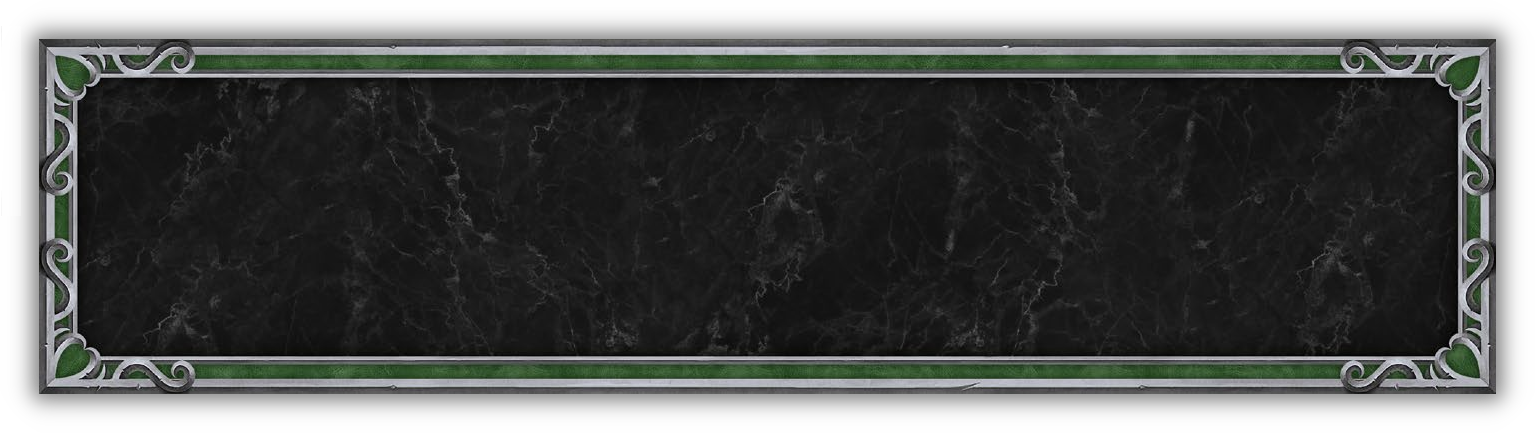
\includegraphics[width=1.055\linewidth, height=0.24\linewidth]{\layout/section_heading.png}}};
        }
        \draw (-6.7, 0) node {\includegraphics[width=0.135\textwidth]{#2}};
      \end{tikzpicture}
    }
  }
  \begin{fullwidth}[leftmargin=0.21\textwidth]
    \begin{center}
      \vspace{1em}
      \vspace{\lang_header_adjustment}
      \section*{\sectionheadertext{#1}}
      \cleardoublepage\phantomsection\addcontentsline{toc}{section}{\protect\numberline{}#1}
      \pagetarget{#1}{}
    \end{center}
  \end{fullwidth}
  \vspace{1.75em}
  \vspace{\lang_header_adjustment}
}
%End of create section heading.

% Add title page for Scenario type
\newcommand{\addscenariogroup}[2]{
  \thispagestyle{empty}
  \cleardoublepage\phantomsection\addcontentsline{toc}{section}{\protect\numberline{}#1}
  \iftoggle{noartbackground}{}{
    \AddToHookNext{shipout/background}{%
      \put (0in,-\paperheight){\includegraphics[width=\paperwidth,height=\paperheight]{\layout/tausta.png}}%
    }
  }
  \begin{tikzpicture}[remember picture, overlay, inner sep=10pt]
    \iftoggle{noartbackground}{}{
      \node(cover)[anchor=center] at (current page.center) {
        \includegraphics[height=\paperheight, keepaspectratio]{#2}
      };
    }
    \node(heading)[anchor=center] at (current page.center) {
      
\includegraphics[width=\linewidth, keepaspectratio]{\layout/grouping_heading.png}
    };
    \node(title)[minimum width = \paperwidth, anchor=center] at (current page.center) {
      \huge\sectionheadertext[bistre]{#1}
    };
  \end{tikzpicture}
}

\newcommand\addheadershadow[2][]{
    % #1: Optional aditional tikz options
    % #2: Name of the node to "decorate"
    \begin{pgfonlayer}{background}
        \path[
           rounded corners=1pt,
           blur shadow={shadow xshift=0pt,
           shadow yshift=0pt,
           shadow blur steps=10,
           shadow blur radius=6pt}, #1]
            ($(#2.north west)+( 0.6pt,0)$) --
            ($(#2.south west)+( 0.6pt,0)$) --
            ($(#2.south east)+(-0.6pt,0)$) --
            ($(#2.north east)+(-0.6pt,0)$) --
        cycle;
        \path[rounded corners,
           blur shadow={shadow xshift=0pt,
           shadow yshift=0pt,
           shadow blur steps=10,
           shadow blur radius=6pt}, #1]
            ($(#2.north west)+(-1.3pt,-3pt)$) --
            ($(#2.south west)+(-1.3pt, 3pt)$) --
            ($(#2.south east)+( 1.3pt, 3pt)$) --
            ($(#2.north east)+( 1.3pt,-3pt)$) --
            cycle;
    \end{pgfonlayer}
}

% Four mandatory params
% - [optional] set to "subsection" or any other Level if you want to have this as a subsection in TOC
% - Lines of Campaign Name (1-2 according to the name length)
% - Campaign Name
% - Scenario Name
% - Icon
%
% TODO: possibly replace the whole \addsection with this
\newcommand{\addscenariosection}[5][section]{
  \sodef\sotitle{}{0.2em}{0.6em}{1.2em}
  \def\oneliner{\equal{#2}{1}}

  \vspace*{-5.72em}
  \hspace*{-1.3em}
  \makebox[0pt][l]{
  \raisebox{-\totalheight}[0pt][7pt]{
    \ifthenelse{\oneliner}{\def\yscale{1}}{\def\yscale{1.3}}
      \begin{tikzpicture}
        \iftoggle{noartbackground}{
          \draw (0, 0) node[inner sep=0, yscale=\yscale] (header){\makebox[1.015\textwidth][c]{
\includegraphics[width=1.055\linewidth, height=0.24\linewidth]{\layout/section_heading_monochrome.png}}};
        }{
          \draw (0, 0) node[inner sep=0, yscale=\yscale] (header){\makebox[1.015\textwidth][c]{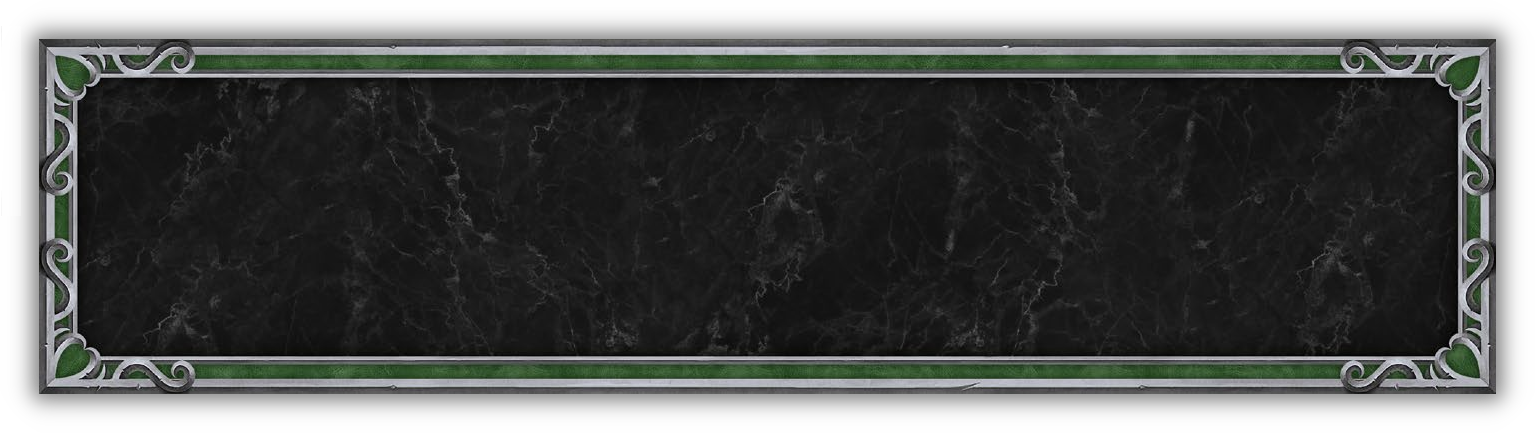
\includegraphics[width=1.055\linewidth, height=0.24\linewidth]{\layout/section_heading.png}}};
        }
        \draw (-6.7, 0) node {\includegraphics[width=0.135\textwidth]{#5}};
      \end{tikzpicture}
    }
  }
  \begin{fullwidth}[leftmargin=0.21\textwidth]
    \begin{center}
      \vspace{\lang_header_adjustment}
      \vspace{-12pt}
      \section*{\sectionheadertext{\small{\sotitle{#3}}}}
      \vspace{\lang_header_adjustment}
      \vspace{-10pt}
      \section*{\sectionheadertext{#4}}
      \ifthenelse{\oneliner}{}{\vspace{14pt}}
      \cleardoublepage\phantomsection\addcontentsline{toc}{#1}{\protect\numberline{} {} {} {} {}#4}
      \pagetarget{#4}{}
    \end{center}
  \end{fullwidth}
  \ifthenelse{\oneliner}{\vspace{1.75em}}{\vspace{0.75em}}
  \vspace{\lang_header_adjustment}
}

% Apply language-specific subsection spacings if defined
\ifdefined\subsectionspacing
  \subsectionspacing{}
\fi

\newcommand\picdims[4][]{%
  \setbox0=\hbox{\includegraphics[#1]{#4}}%
  \clipbox{.5\dimexpr\wd0-#2\relax{} %
    .5\dimexpr\ht0-#3\relax{} %
    .5\dimexpr\wd0-#2\relax{} %
    .5\dimexpr\ht0-#3\relax}{\includegraphics[#1]{#4}}}

\tikzset{
  thick/.style=      {line width=1.3pt},
  very thick/.style= {line width=1.7pt},
  ultra thick/.style={line width=2.2pt}
}

\definecolor{borderoutyellow}{HTML}{DBCA86}
\definecolor{borderinyellow}{HTML}{B09E69}
\definecolor{bordermidyellow}{HTML}{6f6749}
% Create note box
\providecommand{\notefont}[0]{\liberation\selectfont}
\newcommand{\note}[2]{
  \begin{tikzpicture}
    \draw (0, 0) node[inner sep=0] {\makebox[\linewidth][c]{\picdims[width=\linewidth]{\linewidth}{#1\baselineskip}{\layout/table-background.jpg}}};
    \draw [borderoutyellow, very thick] (current bounding box.north west) rectangle (current bounding box.south east);
    \draw [borderinyellow, thick] ([xshift=+2.8pt, yshift=-2.8pt] current bounding box.north west) rectangle ([xshift=-2.8pt, yshift=2.8pt] current bounding box.south east);
    \node at (current bounding box.center) {
      \begin{varwidth}{0.85\linewidth}
      \notefont{
        \color{arylideyellow}
        \hypersetup{linkcolor=amber}
        #2
        \hypersetup{linkcolor=goldenbrown}
      }
      \end{varwidth}
    };
    \begin{pgfonlayer}{background}
      \begin{scope}[blend mode=multiply]
        \draw [shade, blur shadow={shadow opacity=15}] (current bounding box.north west) rectangle (current bounding box.south east);
      \end{scope}
    \end{pgfonlayer}
  \end{tikzpicture}
}

% Create Heroes-styled framed canvas for a table. Accepts three arguments:
% 1) [Optional] Drop shadow description. Use [] as the first arg to delete it.
% 2) Height specified in verses (lines of text)
% 3) Table contents like title and tabularx environment
\newcommand{\hommtable}[3][shade, blur shadow={shadow opacity=15}]{
  \begin{tikzpicture}
    \iftoggle{noartbackground}{
      \node[inner sep=0, minimum width=\linewidth, minimum height=#2\baselineskip] at (0,0) {};
    }{
      \draw (0, 0) node[inner sep=0] {\makebox[\linewidth][c]{\picdims[width=\linewidth]{\linewidth}{#2\baselineskip}{\layout/table-background.jpg}}};
    }
    \draw [bordermidyellow, thick] ([xshift=+1pt, yshift=-1pt] current bounding box.north west) rectangle ([xshift=-1pt, yshift=1pt] current bounding box.south east);
    \draw [borderoutyellow, thick] (current bounding box.north west) rectangle (current bounding box.south east);
    \draw [borderinyellow, thick] ([xshift=+3pt, yshift=-3pt] current bounding box.north west) rectangle ([xshift=-3pt, yshift=3pt] current bounding box.south east);
    \node at (current bounding box.center) {
      \begin{varwidth}{0.95\linewidth}
      \notefont{
        \bgroup
        \iftoggle{noartbackground}{}{
          \color{arylideyellow}
          \hypersetup{linkcolor=amber}
        }
        \setlength{\tabcolsep}{0.3em}
        #3
        \egroup
      }
      \end{varwidth}
    };
    \begin{pgfonlayer}{background}
      \begin{scope}[blend mode=multiply]
        \draw [#1] (current bounding box.north west) rectangle (current bounding box.south east);
      \end{scope}
    \end{pgfonlayer}
  \end{tikzpicture}
}
% End of Heroes-styled canvas definition.

% Redefinition of the table for mutlicol enviromnents
\newcommand{\hommtablemulticol}[3][shade, blur shadow={shadow opacity=15}]{
  \begin{tikzpicture}
    \iftoggle{noartbackground}{
      \node[inner sep=0, minimum width=\linewidth, minimum height=#2\baselineskip] at (0,0) {};
    }{
      \draw (0, 0) node[inner sep=0] {\makebox[\linewidth][c]{\picdims[width=\linewidth]{\linewidth}{#2\baselineskip}{\layout/table-background-multicol.jpg}}};
    }
    \draw [bordermidyellow, thick] ([xshift=+1pt, yshift=-1pt] current bounding box.north west) rectangle ([xshift=-1pt, yshift=1pt] current bounding box.south east);
    \draw [borderoutyellow, thick] (current bounding box.north west) rectangle (current bounding box.south east);
    \draw [borderinyellow, thick] ([xshift=+3pt, yshift=-3pt] current bounding box.north west) rectangle ([xshift=-3pt, yshift=3pt] current bounding box.south east);
    \node at (current bounding box.center) {
      \begin{varwidth}{0.95\linewidth}
      \notefont{
        \bgroup
        \iftoggle{noartbackground}{}{
          \color{arylideyellow}
          \hypersetup{linkcolor=amber}
        }
        \setlength{\tabcolsep}{0.3em}
        #3
        \egroup
      }
      \end{varwidth}
    };
    \begin{pgfonlayer}{background}
      \begin{scope}[blend mode=multiply]
        \draw [#1] (current bounding box.north west) rectangle (current bounding box.south east);
      \end{scope}
    \end{pgfonlayer}
  \end{tikzpicture}
}

\definecolor{darkcellborder}{HTML}{634831}
\definecolor{darkcellbg}{HTML}{20160C}

\newcommand{\darkcell}[2][0.9]{
  \begin{tikzpicture}
    \filldraw[line width=1.0pt, fill=darkcellbg, fill opacity=0.5, draw=darkcellborder] (0, 0) rectangle (\linewidth, #1);
    \node[text width=\linewidth, align=center] at (current bounding box.center) {\textbf{#2}};
  \end{tikzpicture}
}

\newcommand{\darkcellleft}[2][0.9]{
  \begin{tikzpicture}
    \filldraw[line width=1.0pt, fill=darkcellbg, fill opacity=0.5, draw=darkcellborder] (0, 0) rectangle (\linewidth, #1);

    \node[text width=\linewidth, align=left] at (current bounding box.center) {
      \leftskip=0.4em
      \rightskip=0pt plus 1fil
      \textbf{#2}\\
    };
  \end{tikzpicture}
}

\definecolor{lightcellborder}{HTML}{77543e}
\definecolor{lightcellbg}{HTML}{20160C}

\newcommand{\lightcell}[2][0.9]{
  \begin{tikzpicture}
    \filldraw[line width=1.0pt, fill=\iftoggle{noartbackground}{white}{lightcellbg}, fill opacity=0.25, draw=lightcellbg, fill opacity=0.25, draw=lightcellborder] (0, 0) rectangle (\linewidth, #1);
    \node[text width=\linewidth, align=center] at (current bounding box.center) {\iftoggle{noartbackground}{}{\color{white}}#2};
  \end{tikzpicture}
}

\newcommand{\lightcellleft}[2][0.9]{
  \begin{tikzpicture}
    \filldraw[line width=1.0pt, fill=\iftoggle{noartbackground}{white}{lightcellbg}, fill opacity=0.25, draw=lightcellbg, fill opacity=0.25, draw=lightcellborder] (0, 0) rectangle (\linewidth, #1);
    \node[text width=\linewidth, align=left] at (current bounding box.center) {
      \iftoggle{noartbackground}{}{\color{white}}
      \leftskip=0.4em
      \rightskip=0pt plus 1fil
      #2\\
    };
  \end{tikzpicture}
}

% Commands to be used for automation generating printable version
\newcommand{\pagetarget}[2]{\label{#1}\hypertarget{#1}{#2}}
\newcommand{\pagelink}[2]{\hyperlink{#1}{#2}\iftoggle{printable}{ \textmd{(\pageshorthand\,\pageref{#1})}}{}}

% Command for overlay circled text
\definecolor{goblin}{HTML}{3b7c33}
\newcommand\encircle[1]{%
  \tikz[baseline=(X.base)]
  \node (X) [draw=white, shape=circle, inner sep=0, fill=goblin, text=white, blur shadow={shadow blur steps=5}] {\strut \textbf{#1}};%
}

% Background
\AddToHook{shipout/background}{%
  \iftoggle{noartbackground}{}{
    \put (0in,-\paperheight){\includegraphics[width=\paperwidth,height=\paperheight]{\layout/tausta.png}}
  }
  \put (0in,-\paperheight){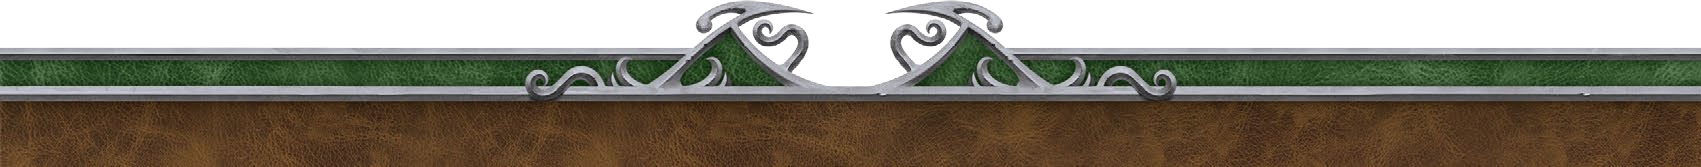
\includegraphics[width=\paperwidth,height=0.05\paperheight]{\layout/bottom.png}}
}

\NewCommandCopy\hrefwithoutfootnote\href
\iftoggle{printable}{
  \renewcommand{\href}[2]{\hrefwithoutfootnote{#1}{#2}\footnote{#1}\enlargethispage{\baselineskip}}
}

\begin{document}

% !TeX spellcheck = en_US
\thispagestyle{empty}
\begin{tikzpicture}[remember picture, overlay, inner sep=10pt]
  \iftoggle{noartbackground}{}{
    \node(cover)[anchor=center] at (current page.center) {
      \includegraphics[height=\paperheight, keepaspectratio]{\layout/cover.jpg}
    };
  }
  \node(title)[minimum width = \paperwidth, anchor=center, yshift=\dimexpr-10em\relax] at (current page.north) {
    \includegraphics[width=0.6\paperwidth]{\layout/cover_title.png}
  };
  \node(subtitle)[anchor=center, yshift=12em] at (current page.south) {
    
\includegraphics[width=0.6\paperwidth]{\layout/cover_subtitle.png}
  };
\end{tikzpicture}

% Render phantom SVGs before their use in tabular env
\phantom{
  \includesvg[height=0.1px]{\svgs/bronze.svg}
  \includesvg[height=0.1px]{\svgs/bronze.svg}
  \includesvg[height=0.1px]{\svgs/silver.svg}
  \includesvg[height=0.1px]{\svgs/golden.svg}
  \includesvg[height=0.1px]{\svgs/azure.svg}
  \includesvg[height=0.1px]{\svgs/gold.svg}
  \includesvg[height=0.1px]{\svgs/building_materials.svg}
  \includesvg[height=0.1px]{\svgs/valuables.svg}
  \includesvg[height=0.1px]{\svgs/attack-yellow.svg}
  \includesvg[height=0.1px]{\svgs/defense-yellow.svg}
  \includesvg[height=0.1px]{\svgs/damage-yellow.svg}
}


% !TeX spellcheck = en_US
\title{\includegraphics[width=6cm]{\images/title.png}\\Fan-Made Mission Book}

\author{By The Community}
\maketitle

\begin{center}
  \iftoggle{githubbuild}{
    \getenv[\githubsha]{GITHUB_SHA}
    This is an unreleased version built on GitHub from commit \hrefwithoutfootnote{\repourl}{\StrLeft{\githubsha}{7}}.
  }{
    Version \input{.version}
  }

  \bigbreak

  This is a community-driven project, which has a \hrefwithoutfootnote{\repourl}{GitHub repository}.
  Everyone is welcome to contribute Scenarios, make changes, and fix errors.

  \bigbreak

  \begin{multicols}{2}
    \bigbreak
    \centering
    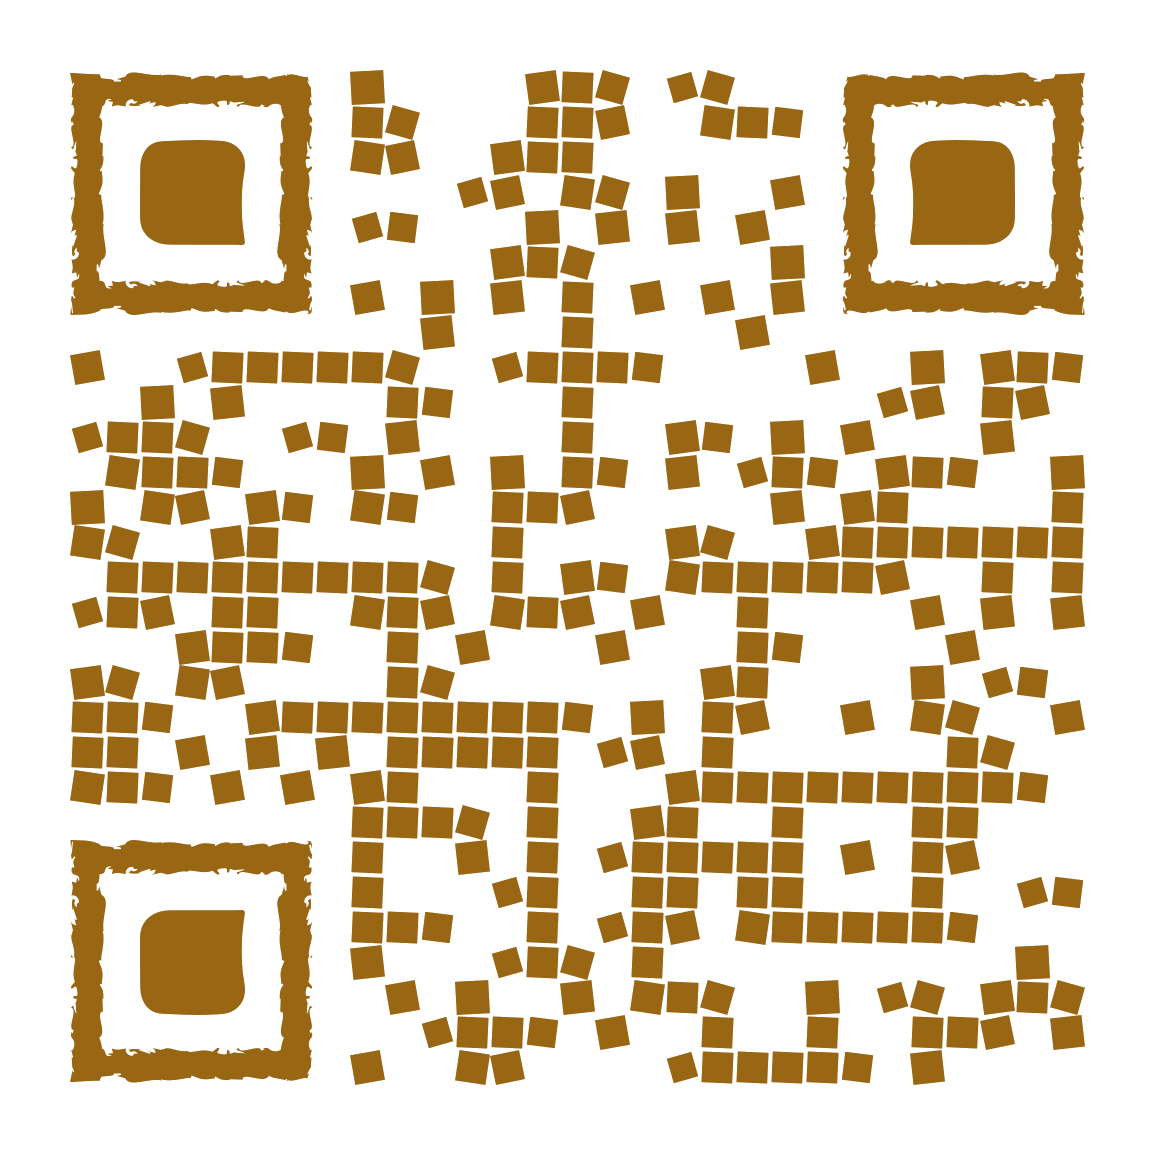
\includegraphics[width=0.8\linewidth]{\qr/discord.png}\\
    Scan to join the Heroes III Board Game community \textbf{Discord} server.\\
    \href{\discordurl}{\discordurl}

    \columnbreak
    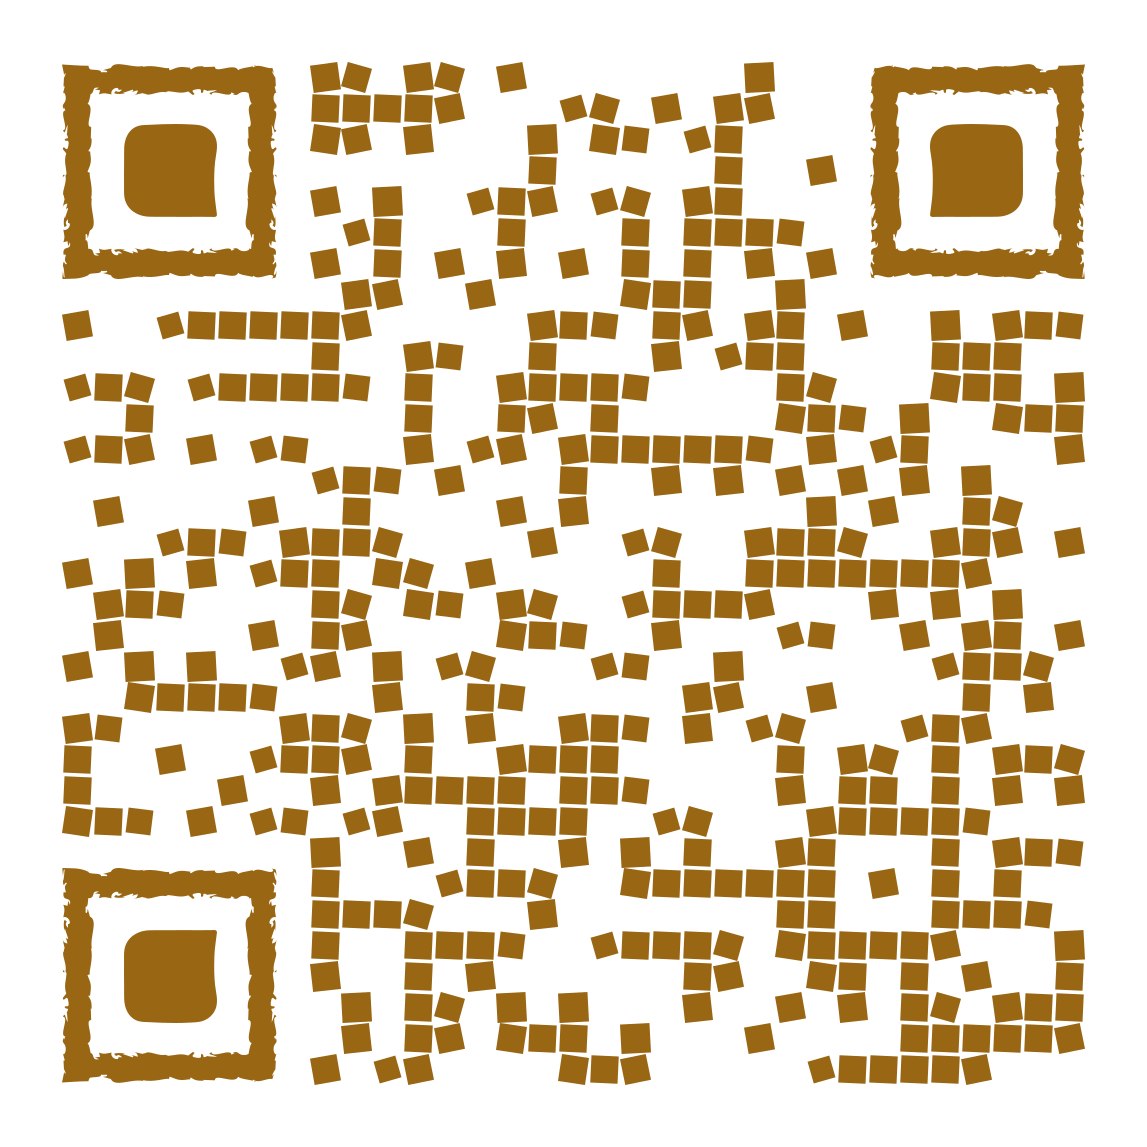
\includegraphics[width=0.8\linewidth]{\qr/github.png} \\
    Scan to open \textbf{GitHub} repository. \\
    \href{\repourl}{\repourl}
  \end{multicols}
\end{center}

\iftoggle{noartbackground}{}{
  \AddToHookNext{shipout/background}{
    \put (0in,-\paperheight){\includegraphics[width=\paperwidth,height=\paperheight]{\layout/tausta.png}}
  }
}
\thispagestyle{empty}
\begin{tikzpicture}[remember picture, overlay]
  \node(cover)[anchor=center, yshift=9em] at (current page.south) {
    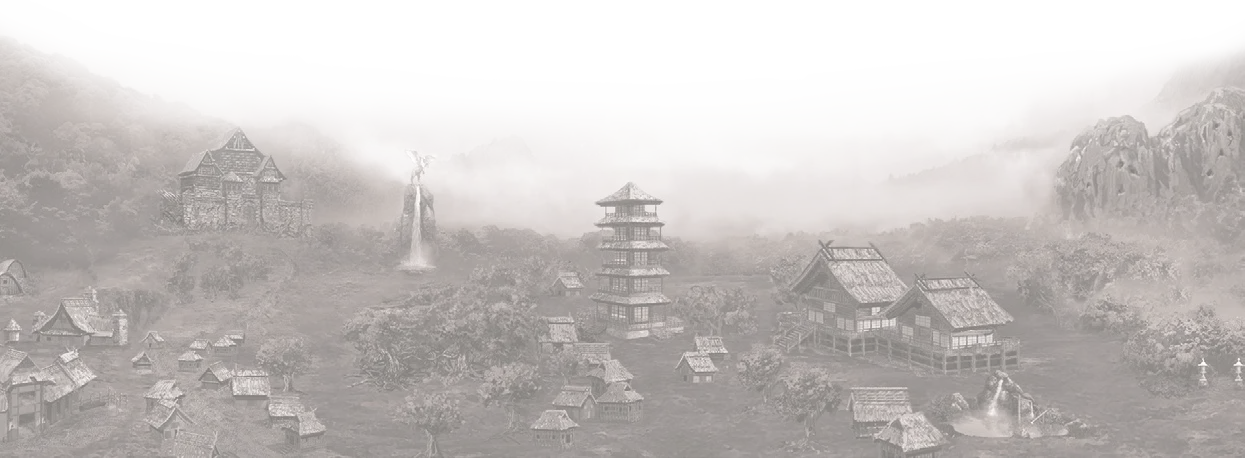
\includegraphics[width=1.01\paperwidth, keepaspectratio]{\layout/rampart_background.png}
  };
\end{tikzpicture}

\clearpage
\begin{multicols*}{2}
\tableofcontents
\vspace*{\fill}
\columnbreak
\vspace{-3em}
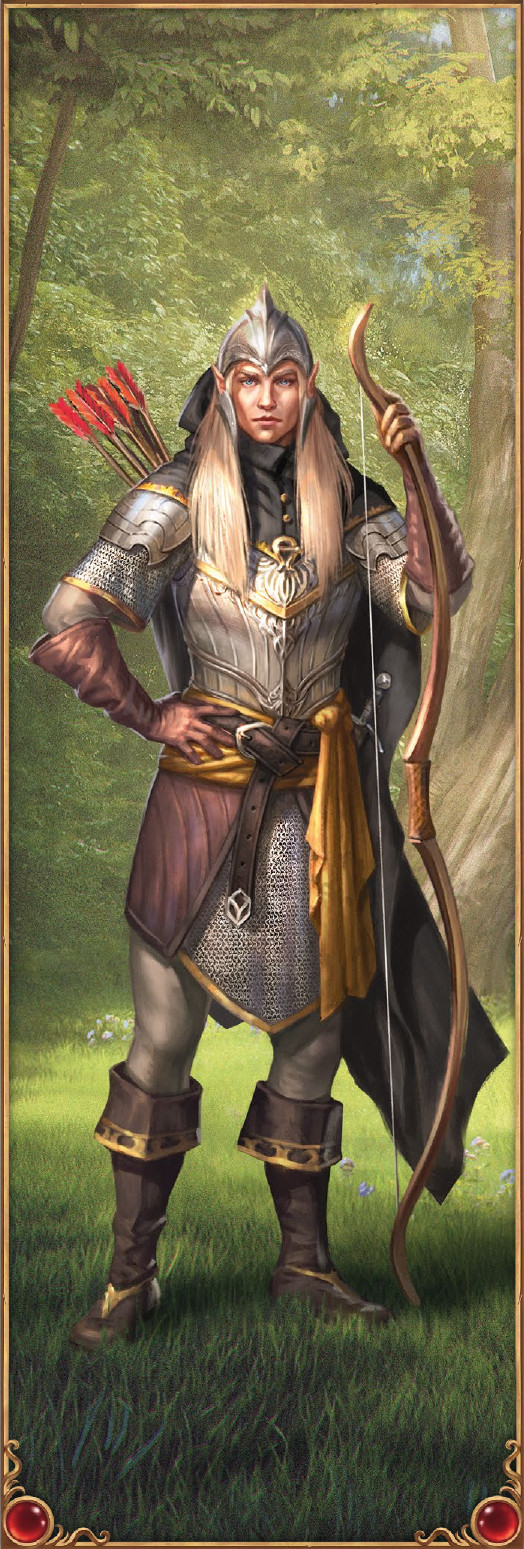
\includegraphics[width=\linewidth]{\art/elf.jpg}

\end{multicols*}


% !TeX spellcheck = en_US
\addsection{What to Play}{\images/forgetfulness.png}

\begin{multicols}{2}

Follow these suggestions if you're not sure which scenario is best for you.

\subsection*{Cooperative Mode}

If you're new to the game and want to try \textbf{learning the rules}, start with \pagelink{Emerald Island}{Emerald Island}.
For a big adventure for \textbf{up to 6 players} with an epic battle at the end, try \pagelink{Titans' Stronghold}{Titans' Stronghold}.
For more tactical play for two players, try \pagelink{Sentinels}{Sentinels}.

\subsection*{Clash Mode}

If you'd like to play a 2- or 4-player ``capture the Grail'' scenario with interesting twists, try \pagelink{Bloody Grail}{Bloody Grail}.
For an exciting boss fight for 3 players, choose \pagelink{The Hunt}{The Hunt}.
For an inevitable epic battle between two players with a possible siege, play \pagelink{Dragoncurse Castle}{Dragoncurse Castle}.

\subsection*{Campaign}

There is a 3-scenario Inferno \pagelink{1. A Devilish Plan}{Dungeons and Devils} Campaign at the end if you prefer solo play.

\subsection*{Recommendations}

For information regarding your play time, strategizing, and custom rules, checkout out \pagelink{Recommendations}{recommendations} at the and of this book.

\end{multicols}

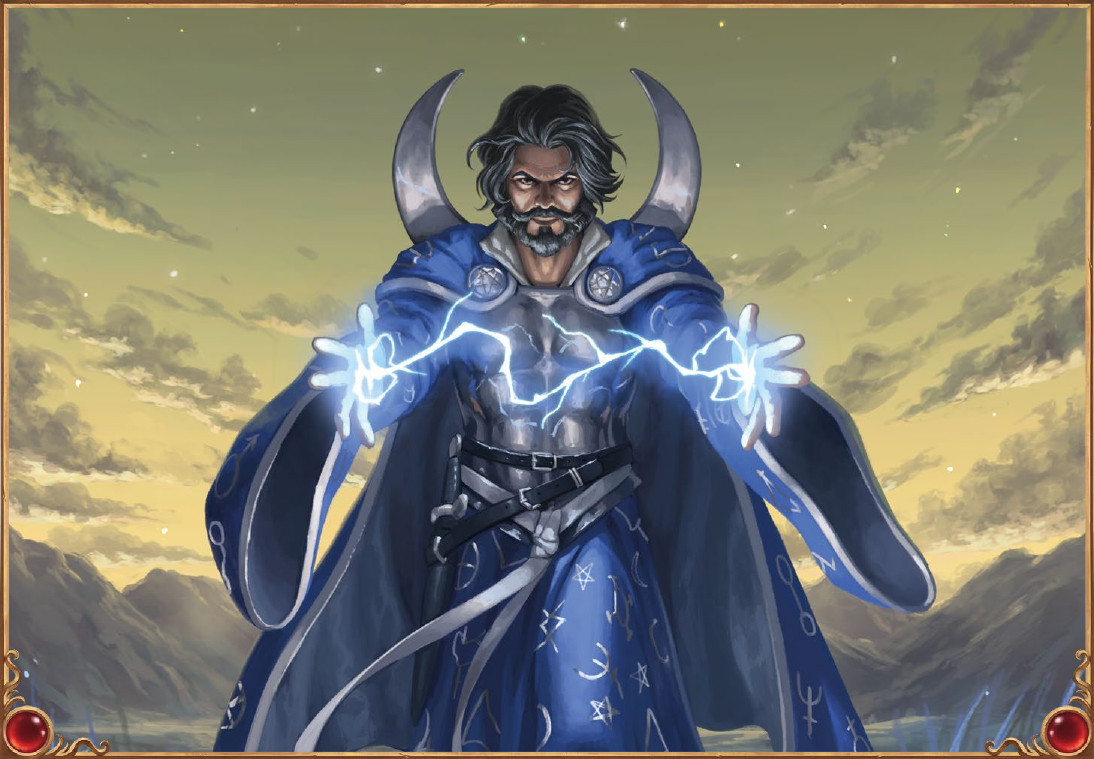
\includegraphics[width=\linewidth]{\art/enchanter.jpg}


\addscenariogroup{Cooperative Scenarios}{\layout/coops.png}

\clearpage

\input{\coops/sentinels.tex}

\clearpage

\input{\coops/titans_stronghold.tex}

\clearpage

\input{\coops/emerald_island.tex}


\addscenariogroup{\clashtitle}{\layout/clash.png}

\clearpage

\input{\clashpath/bloody_grail.tex}

\clearpage

% \input{\clashpath/the_hunt.tex}


% !TeX spellcheck = en_US
\addsection{Random Scenario}{\images/random.png}

\begin{multicols}{2}

\textit{As dice roll and fortunes shift, the lands of Antagarich spread before you in all their splendor.
  Your destiny follows these celestial rolls, each battle and treasure determined by chance.
  Will you emerge victorious in this battle royale, claim the sacred grail, or stand alone as the king of the hill when the final die settles?  % no-check-caps
}

Instead of playing a specific Scenario, you can follow these guidelines to create a random one.
Of course, you can adjust everything at will.

\subsection*{\MakeUppercase{Scenario Type}}

Choose one of the following types for your play:

\textbf{Free-for-All} -- Win by eliminating your opponents or gaining more Victory Points (VPs) than them.
VPs are counted in accordance to the Tournament book.
Additionally, you get:
\begin{itemize}
  \item 5 VPs for flagging a Dragon Utopia for the first time.
  \item 2 VPs for controlling the Dragon Utopia at the end of the game.
  \item 5 VPs for bringing the Grail to your Faction Town \textit{OR} 3 VPs for owning the Grail  at the end of the game.
\end{itemize}

\textbf{King of the Hill} -- Start a map with a Dragon Utopia in the middle.
You don't need to fight the Level 7 Combat to capture it.
You get 1 VP for each Round you hold the Dragon Utopia under your control, no VPs from anything else.

\textbf{Capture the Grail} -- Start a map with the Grail in the middle.
Standard Grail rules apply: spend 2 \svgeven{movement} to dig it up, and bring it to your Town.
\vspace*{\fill}
\columnbreak

\subsection*{\MakeUppercase{Map Size}}

\textbf{Small (S) Map:} 8 Rounds, and give every player:
\begin{itemize}
  \item 1 × Starting (I) Map Tile
  \item 2 × Far (II-III) Map Tile
\end{itemize}

\textbf{Medium (M) Map:} 12 Rounds, and give every player:
\begin{itemize}
  \item 1 × Starting (I) Map Tile
  \item 2 × Far (II-III) Map Tile
  \item 1 × Near (IV-V) Map Tile
\end{itemize}

\textbf{Large (XL) Map:} 16 Rounds, and give every player:
\begin{itemize}
  \item 1 × Starting (I) Map Tile
  \item 2 × Far (II-III) Map Tile
  \item 2 × Near (IV-V) Map Tile
\end{itemize}

\medskip

\hommtablemulticol[]{19}{
  \centering
  \medskip
  \textbf{Central Map Tile(s)}\\
  \bigskip
  \hspace{-0.7em}
  \begin{tabularx}{0.99\linewidth}{p{1.7em}>{\centering\arraybackslash}X>{\centering\arraybackslash}X>{\centering\arraybackslash}X} & \darkcell[1.4]{Free-for-All} & \darkcell[1.4]{King of the Hill} & \darkcell[1.4]{Capture the Grail} \\
    \darkcell[1.8]{S}
    & \lightcell[1.8]{
\includegraphics[width=0.75\linewidth]{\maps/near-tile.png}}
    & \multirow{3}{*}[7.6ex]{\parbox{\linewidth}{\centering\lightcell[6.19]{
\includegraphics[width=0.75\linewidth]{\maps/center-tile.png} with a Dragon Utopia (C1 or C3)}}}
    & \multirow{3}{*}[7.6ex]{\parbox{\linewidth}{\centering\lightcell[6.19]{
\includegraphics[width=0.75\linewidth]{\maps/center-tile.png} with a\linebreak Grail\linebreak (C2 or C4)}}} \\
    \darkcell[2.2]{M}
    & \lightcell[2.2]{
\includegraphics[width=0.95\linewidth]{\maps/medium.png}}
    &
    & \\
    \darkcell[1.8]{XL}
    & \lightcell[1.8]{
\includegraphics[width=0.75\linewidth]{\maps/center-tile.png}}
    &
    & \\
  \end{tabularx}
}

\end{multicols}

\vspace{-3\baselineskip}

\subsection*{\MakeUppercase{Map Setup}}

\definecolor{castlebg}{RGB}{25,85,196}
\definecolor{infernobg}{RGB}{190,21,38}
\definecolor{rampartbg}{RGB}{53,192,56}

First, place the Central Map Tile(s) for your Scenario type and size in the middle.
Decide player order before placing the remaining Tiles.
In reverse player order, each player places one Tile in descending level (Near \rightarrow\ Far \rightarrow\ Starting).  % no-check-caps
Every new Tile needs to connect to at least one existing Tile.

The following \textbf{example} shows building the map for a \textbf{3-player XL Free-for-All}, with player 1 playing as \textcolor{rampartbg}{\textbf{Rampart}}, player 2 as \textcolor{infernobg}{\textbf{Inferno}}, and player 3 as \textcolor{castlebg}{\textbf{Castle}}.
First, put the Center (VI-VII) Map Tile in the middle, and then proceed to distribute Near (IV-V) Map Tiles in the following order:

\bigskip

% Create a command for player images with horizontal padding
\newcommand{\playerimage}[2]{%
  \begin{minipage}[t]{0.28\textwidth} % Slightly narrower to create padding
    \centering
    \includegraphics[width=0.9\linewidth]{#1} % Images at 90% of column width for padding
    \captionof{figure}{\large\textbf{#2}}
  \end{minipage}%
}

\newcommand{\playerarrow}[4]{%
  % #1 = x-offset from current position
  % #2 = y-offset from current position
  % #3 = rotation angle in degrees
  % #4 = arrow color
  \tikz[remember picture, overlay, baseline=(current bounding box.base)] {
    \coordinate (here) at (0,0);
    \draw[-Triangle, ultra thick, #4, opacity=0.8]
      ([shift={(#1,#2)}]here) -- ++({#3}:0.8cm);
  }%
}

% Save the content in a box to measure its dimensions
\newsavebox{\contentbox}
\begin{lrbox}{\contentbox}
\begin{minipage}{\textwidth}
  % Header
  \noindent
  \rule{\textwidth}{0pt}
  \hspace{0.01\textwidth} % Add left margin
  \rule{\textwidth}{0pt}
  \begin{minipage}{\textwidth/3}
    \centering
    \textbf{\textcolor{castlebg}{Player 3: Castle}}
  \end{minipage}%
  \hfill
  \begin{minipage}{\textwidth/3}
    \centering
    \hspace{1em}\textbf{\textcolor{infernobg}{Player 2: Inferno}}
  \end{minipage}%
  \hfill
  \begin{minipage}{\textwidth/3}
    \centering
    \hspace{1.5em}\textbf{\textcolor{rampartbg}{Player 1: Rampart}}
  \end{minipage}%
  \vspace{1em}
  % First row
  \noindent
  \hspace{0.01\textwidth} % Add left margin
  \playerimage{\maps/free-for-all-xl-1.png}{1}%
  \playerarrow{-2.8}{0.2}{60}{castlebg}
  \hfill
  \playerimage{\maps/free-for-all-xl-2.png}{2}%
  \playerarrow{-1.5}{0.2}{160}{infernobg}
  \hfill
  \playerimage{\maps/free-for-all-xl-3.png}{3}
  \playerarrow{-4.3}{2.6}{-60}{rampartbg}
  \hspace{0.01\textwidth} % Add right margin
  \begin{center}
    \color{darkgray}{\rule{0.98\textwidth}{0.5pt}}
  \end{center}
  \vspace{1em}

  % Second row
  \noindent
  \hspace{0.01\textwidth} % Add left margin
  \playerimage{\maps/free-for-all-xl-4.png}{4}%
  \playerarrow{-3.2}{3.2}{-30}{castlebg}
  \hfill
  \playerimage{\maps/free-for-all-xl-5.png}{5}%
  \playerarrow{-0.8}{1.4}{210}{infernobg}
  \hfill
  \playerimage{\maps/free-for-all-xl-6.png}{6}
  \playerarrow{-3.6}{1.2}{120}{rampartbg}
  \hspace{0.01\textwidth} % Add right margin
  \begin{center}
    \color{darkgray}{\rule{0.98\textwidth}{0.5pt}}
  \end{center}
\end{minipage}
\end{lrbox}

% Draw the background columns based on content dimensions
\begin{tikzpicture}
  % Calculate content height
  \newlength{\contentheight}
  \setlength{\contentheight}{\ht\contentbox}
  \addtolength{\contentheight}{\dp\contentbox}

  % Draw the background columns with fixed positions and extra padding
  % Moving columns slightly to align better with the padded content
  \fill[castlebg, opacity=0.1] (0.01\textwidth,0) rectangle (0.31\textwidth,-\contentheight);
  \fill[infernobg, opacity=0.1] (0.36\textwidth,0) rectangle (0.66\textwidth,-\contentheight);
  \fill[rampartbg, opacity=0.1] (0.71\textwidth,0) rectangle (0.99\textwidth,-\contentheight);

  % Place the content
  \node[inner sep=0pt, anchor=north west] at (0,0) {\usebox{\contentbox}};
\end{tikzpicture}

\vspace{1em}

Then, keeping the same order, place Far (II-III) Map Tiles, and finally Starting (I) Map Tiles:

\vspace{1em}

\begin{minipage}{\textwidth}
  \noindent
  \hspace{0.01\textwidth} % Add left margin
  \playerimage{\maps/free-for-all-xl-far-1.png}{7}%
  \playerarrow{-4.4}{3.8}{-30}{rampartbg}
  \playerarrow{-3.9}{-0.3}{60}{infernobg}
  \playerarrow{-0.6}{4.0}{-120}{castlebg}
  \hfill
  \playerimage{\maps/free-for-all-xl-far-2.png}{8}%
  \playerarrow{-4.7}{4.3}{-60}{rampartbg}
  \playerarrow{-5.2}{-0.1}{30}{infernobg}
  \playerarrow{-0.9}{4.3}{-150}{castlebg}
  \hfill
  \playerimage{\maps/free-for-all-xl-finish.png}{9}
  \playerarrow{-5.2}{4.3}{-30}{rampartbg}
  \playerarrow{-5.5}{0.9}{30}{infernobg}
  \playerarrow{-0.3}{4.3}{-150}{castlebg}
  \hspace{0.01\textwidth} % Add right margin
\end{minipage}

\begin{center}
  \color{darkgray}{\rule{0.98\textwidth}{0.5pt}}
\end{center}

\pagebreak


\subsection*{\MakeUppercase{Player Setup}}

Choose your \textbf{starting conditions} and \textbf{Town strength}.

\let\origbronze\bronze
\let\origsilver\silver
\let\origgolden\golden
\let\origazure\azure
\renewcommand{\bronze}{\origbronze[12]}
\renewcommand{\silver}{\origsilver[12]}
\renewcommand{\golden}{\origgolden[12]}
\renewcommand{\azure}{\origazure[12]}


\hommtable[]{27}{
  \centering
  \medskip
  \textbf{Starting Conditions}\\
  \bigskip

  \begin{tabularx}{0.99\linewidth}{p{0.12\linewidth}XXXX} & \darkcell{Stingy} & \darkcell{Fair} & \darkcell{Generous}\\
  \darkcell[1.4]{Army}
    & \lightcellleft[1.4]{2 × Few cheapest \bronze\ Units}
    & \lightcellleft[1.4]{Pack of cheap \bronze\ Units \linebreak Few chosen \bronze\ Units}
    & \lightcellleft[1.4]{Pack of chosen \bronze\ Units \linebreak Few cheap \silver\ Units}\\
  \darkcell[1.4]{Starting Resources}
    & \lightcellleft[1.4]{10 \svg{gold}, 3 \svg{building_materials}, 1 \svg{valuables}}
    & \lightcellleft[1.4]{16 \svg{gold}, 5 \svg{building_materials}, 1 \svg{valuables}}
    & \lightcellleft[1.4]{20 \svg{gold}, 8 \svg{building_materials}, 2 \svg{valuables}}\\
  \end{tabularx}

  \bigskip
  {\color{\iftoggle{noartbackground}{black}{darkyellow}}\rule{\textwidth}{0.5pt}}

  \vspace*{1em}
  \textbf{Town Strength}\\
  \bigskip

  \begin{tabularx}{0.99\linewidth}{p{0.12\linewidth}XXXX} & \darkcell{Settlement} & \darkcell{City} & \darkcell{Capitol}\\
  \darkcell[1.4]{Starting Income}
    & \lightcellleft[1.4]{10 \svg{gold}, 0 \svg{building_materials}, 0 \svg{valuables}}
    & \lightcellleft[1.4]{15 \svg{gold}, 0 \svg{building_materials}, 1 \svg{valuables}}
    & \lightcellleft[1.4]{20 \svg{gold}, 2 \svg{building_materials}, 1 \svg{valuables}}\\
  \darkcell[2.0]{Town Buildings}
    & \lightcellleft[2.0]{\bronze\ Dwelling}
    & \lightcellleft[2.0]{\bronze\ Dwelling \linebreak City Hall}
    & \lightcellleft[2.0]{\bronze\ Dwelling \linebreak City Hall \linebreak Citadel}\\
  \end{tabularx}
}

\begin{multicols}{2}

\subsection*{\MakeUppercase{Timed Events}}

\textbf{\nth{1} Round:}
\begin{itemize}
  \item All Heroes gain +1 \svgeven{movement}.
\end{itemize}
\textbf{\nth{6} and \nth{9} Rounds:}
\begin{itemize}
  \item Remove all Black Cubes from every Water Wheel and Windmill on the map.
\end{itemize}
\textbf{\nth{10} Round:}
\begin{itemize}
  \item Player(s) whose Main Hero has the least experience roll 2 \svg{resource}.
\end{itemize}
\textbf{\nth{12} Round:}
\begin{itemize}
  \item Repeat event of Round 6.
\end{itemize}

\columnbreak

\subsection*{\MakeUppercase{Additional Rules}}

\begin{itemize}
  \item When Visiting a an Obelisk, roll 2 \svg{treasure} and choose 1 to resolve.
  \item Players can spend their Build Token at any time to perform Trading Post actions.
  \item Level VII Combat cannot be skipped by Diplomacy or any other means.
\end{itemize}

\vspace*{\fill}

\end{multicols}


\addscenariogroup{\campaignstitle}{\layout/campaigns.png}

\clearpage

\input{campaigns/inferno_devilish_plan.tex}

\clearpage

\input{campaigns/inferno_steadwicks_fall.tex}

% !TeX spellcheck = en_US
\addsection{Recommendations}{\art/haste.png}

\iftoggle{printable}{}{\bigbreak}

\begin{multicols*}{2}
We've compiled some custom rules and best practices to enhance your gaming experience.
Keep in mind that these are just the \textbf{opinions of the authors} of this book.
Enjoy!

\subsection*{Play Time}

You can estimate your \textbf{minimal} play time using the following formula:

\begin{center}
  Play Time $= \boldsymbol{P × R × 5}$ [min]
\end{center}

Where:
\begin{itemize}
  \item[$\textbf{P}$] -- number of players
  \item[$\textbf{R}$] -- number of Rounds
\end{itemize}

For example, if you're playing a 3-player Scenario consisting of 12 Rounds, you can easily calculate that $3 \times 12 \times 5 = 180$.
Your expected minimal play time would be around 3 hours.

To calculate the \textbf{upper bound} of your play time (more realistic if there are inexperienced players), simply double the result.
In this case, that would be 6 hours.

\subsection*{Magic Arrows}

Except for the Magic Arrow, each Spell appears exactly twice in the Spell Deck.
After players prepare their starting M\&M Decks, it is recommended to remove Magic Arrows from the Spell Deck until no more than two remain.

\subsection*{Guaranteed Settlement}

When distributing Far Tiles (II--III) between players, each player's pool of Map Tiles must include one Settlement.

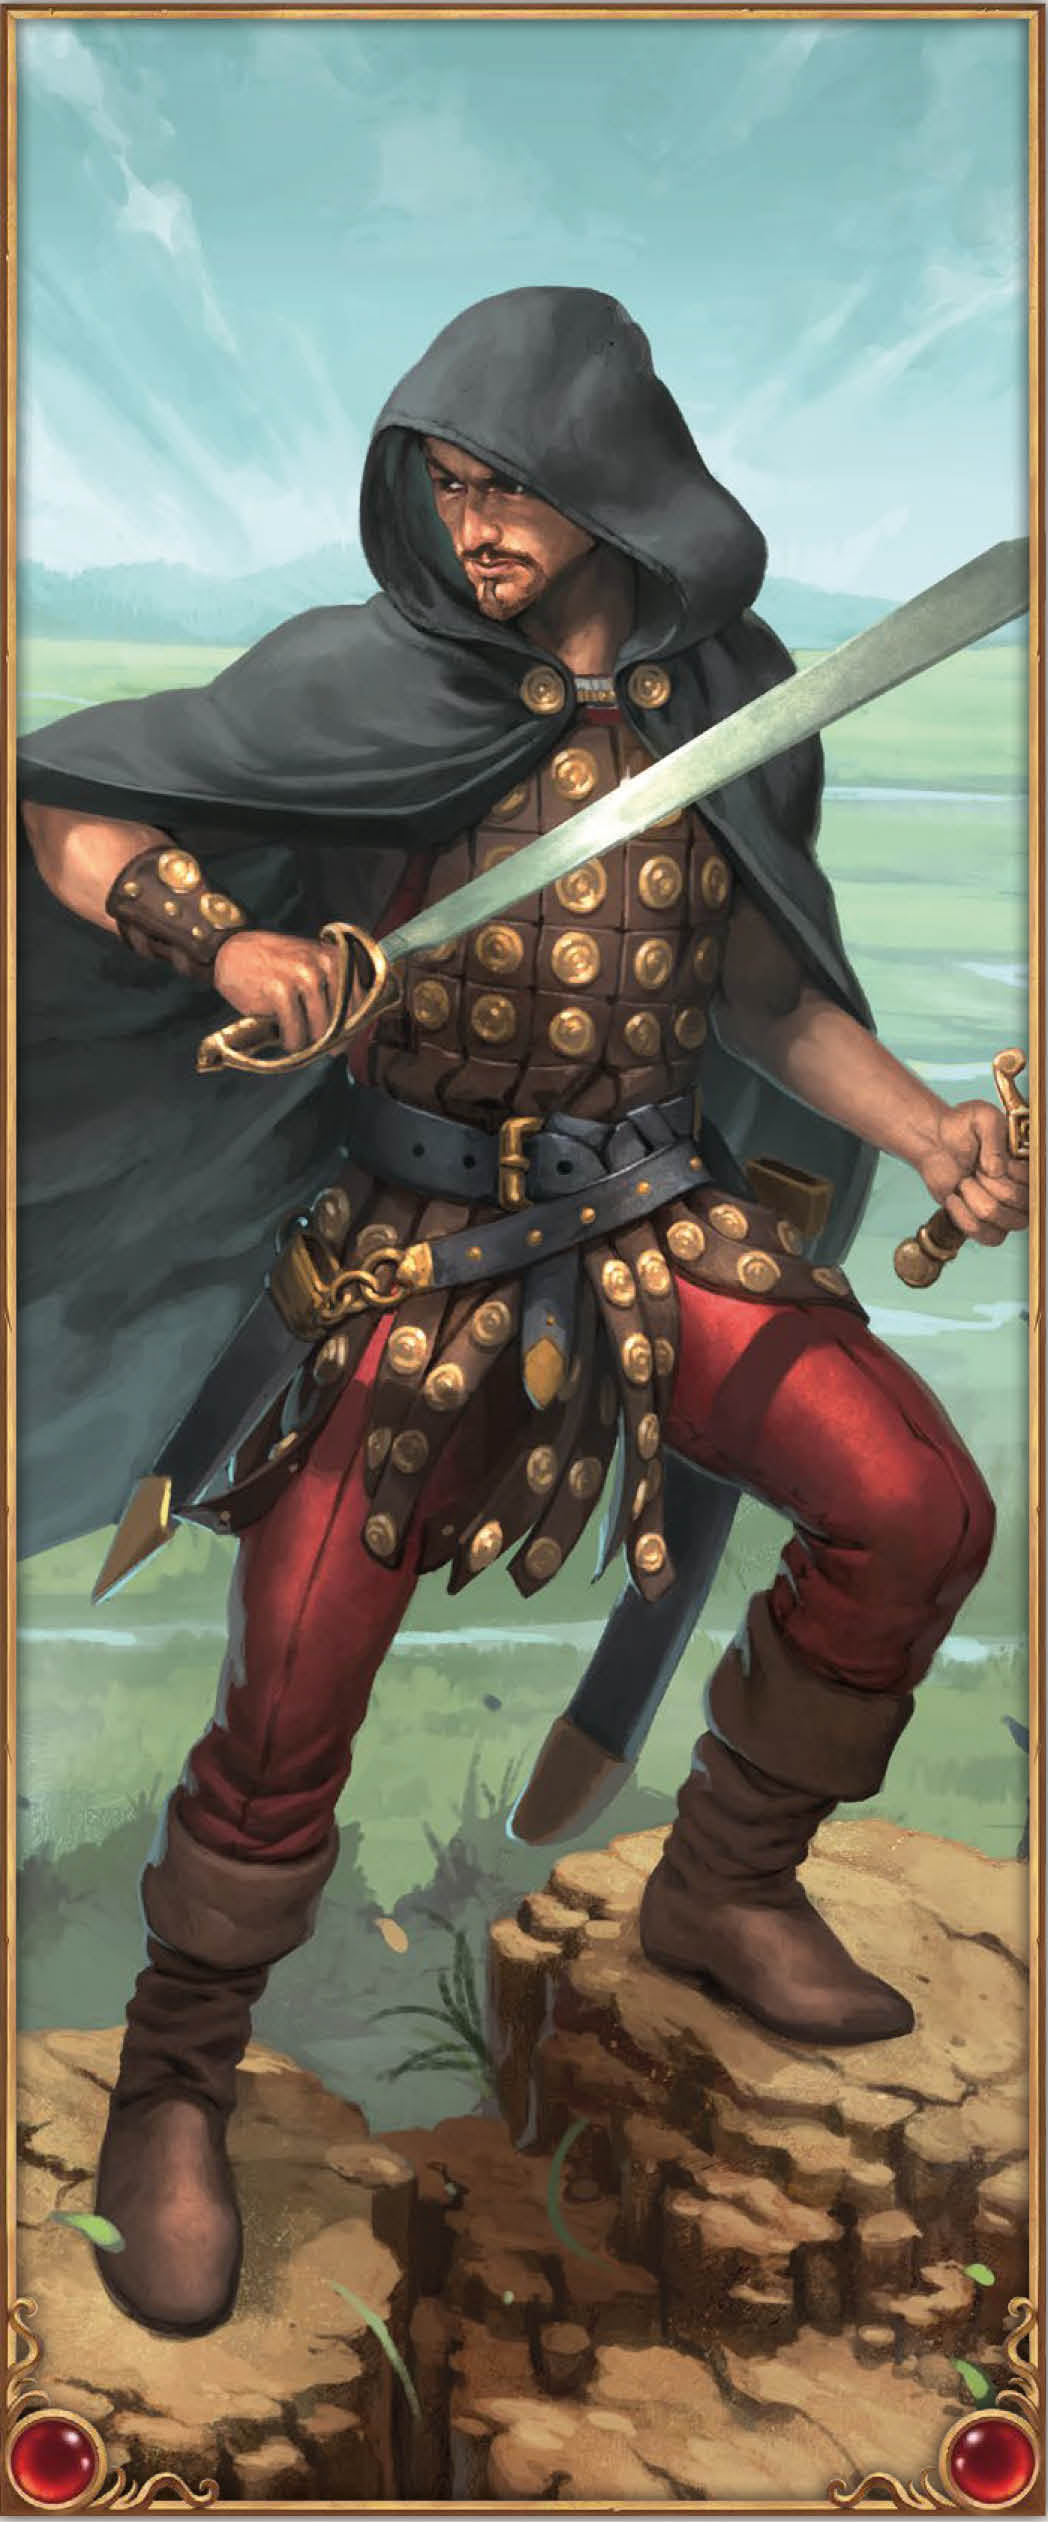
\includegraphics[width=\linewidth]{\art/rogue.jpg}

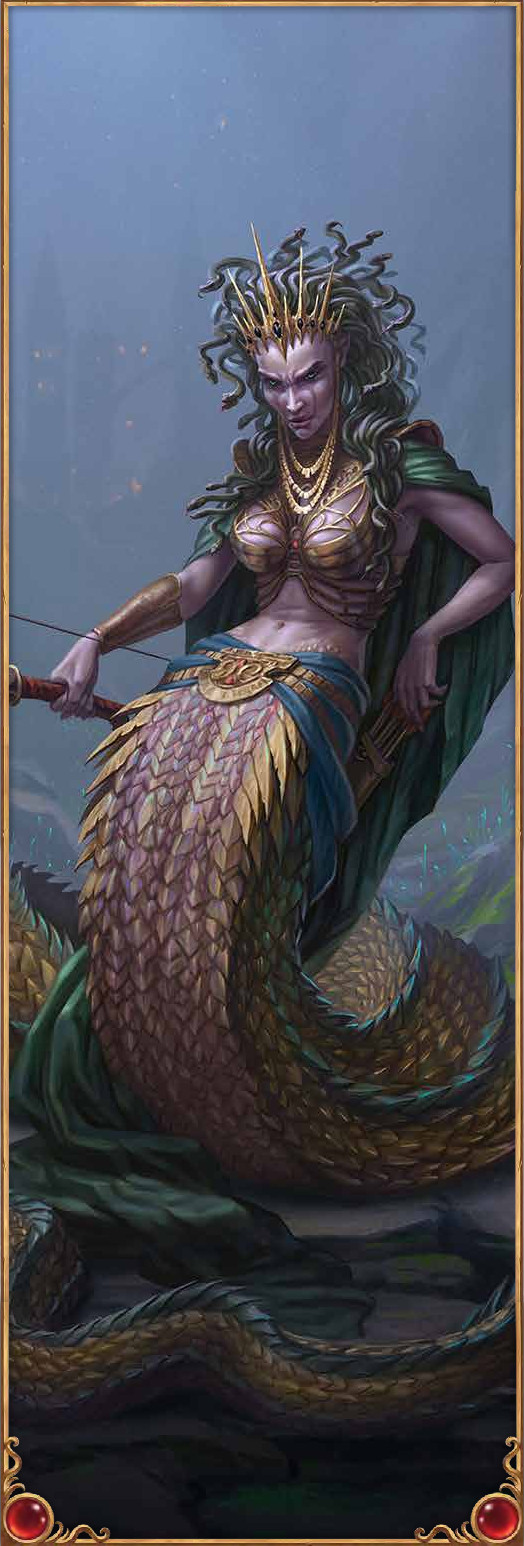
\includegraphics[width=\linewidth]{\art/medusa.jpg}

\subsection*{War Machines as Artifacts}

Shuffle one of each War Machine into the Artifact Deck before the start of the game.
If using the optional Tournament rule of splitting the Artifact Deck, shuffle the War Machines into the Major Artifact Deck.

\subsection*{Round One Mulligan}

At the start of the \nth{1} Round, each player may reshuffle their hand of Cards back into their Deck of Might and Magic and draw a new starting hand of Cards once.

\subsection*{Tier V--VII Combat on Hard+ Difficulty}

Treat Level V--VII Combats as one difficulty step lower when playing on Hard or Impossible.
For example, a Level VII Combat on Hard will be against 2 × \svgunit{azure} Neutral Units.

\subsection*{Trading Post}

Although rules as written state that you can remove only one card from your hand while Visiting a Trading Post, it is recommended to allow removing as many as you like.

\subsection*{Victory Points}

When playing with the optional Victory Points from the Tournament book, the following rules apply (unless overruled by the Scenario):
\begin{itemize}
  \item Faction Towns grant 1 VP.
  \item Possessing the Grail at the end of the match grants 3 VPs. If the Grail was transported to that player's Faction Town, it grants 5 VPs instead.
  \item Capturing a Dragon Utopia grants 3 VPs.
\end{itemize}

\end{multicols*}

\begin{multicols}{2}

\subsection*{Combat with Neutral Units}

During Combat with Neutral Units in clash Scenarios, if a player decides to deploy their Units only on one half (left or right) of the battle Board, the player positioning the Neutral Units must do the same.

Placing Neutral Units far apart only makes the other player waste MPs, which slows the game down.
The exception to this rule is when there are three Neutral \svg{unit_ground} or \svg{unit_flying} Units to position, as all of them must go to the front line.
See examples that follow.

\begin{center}
  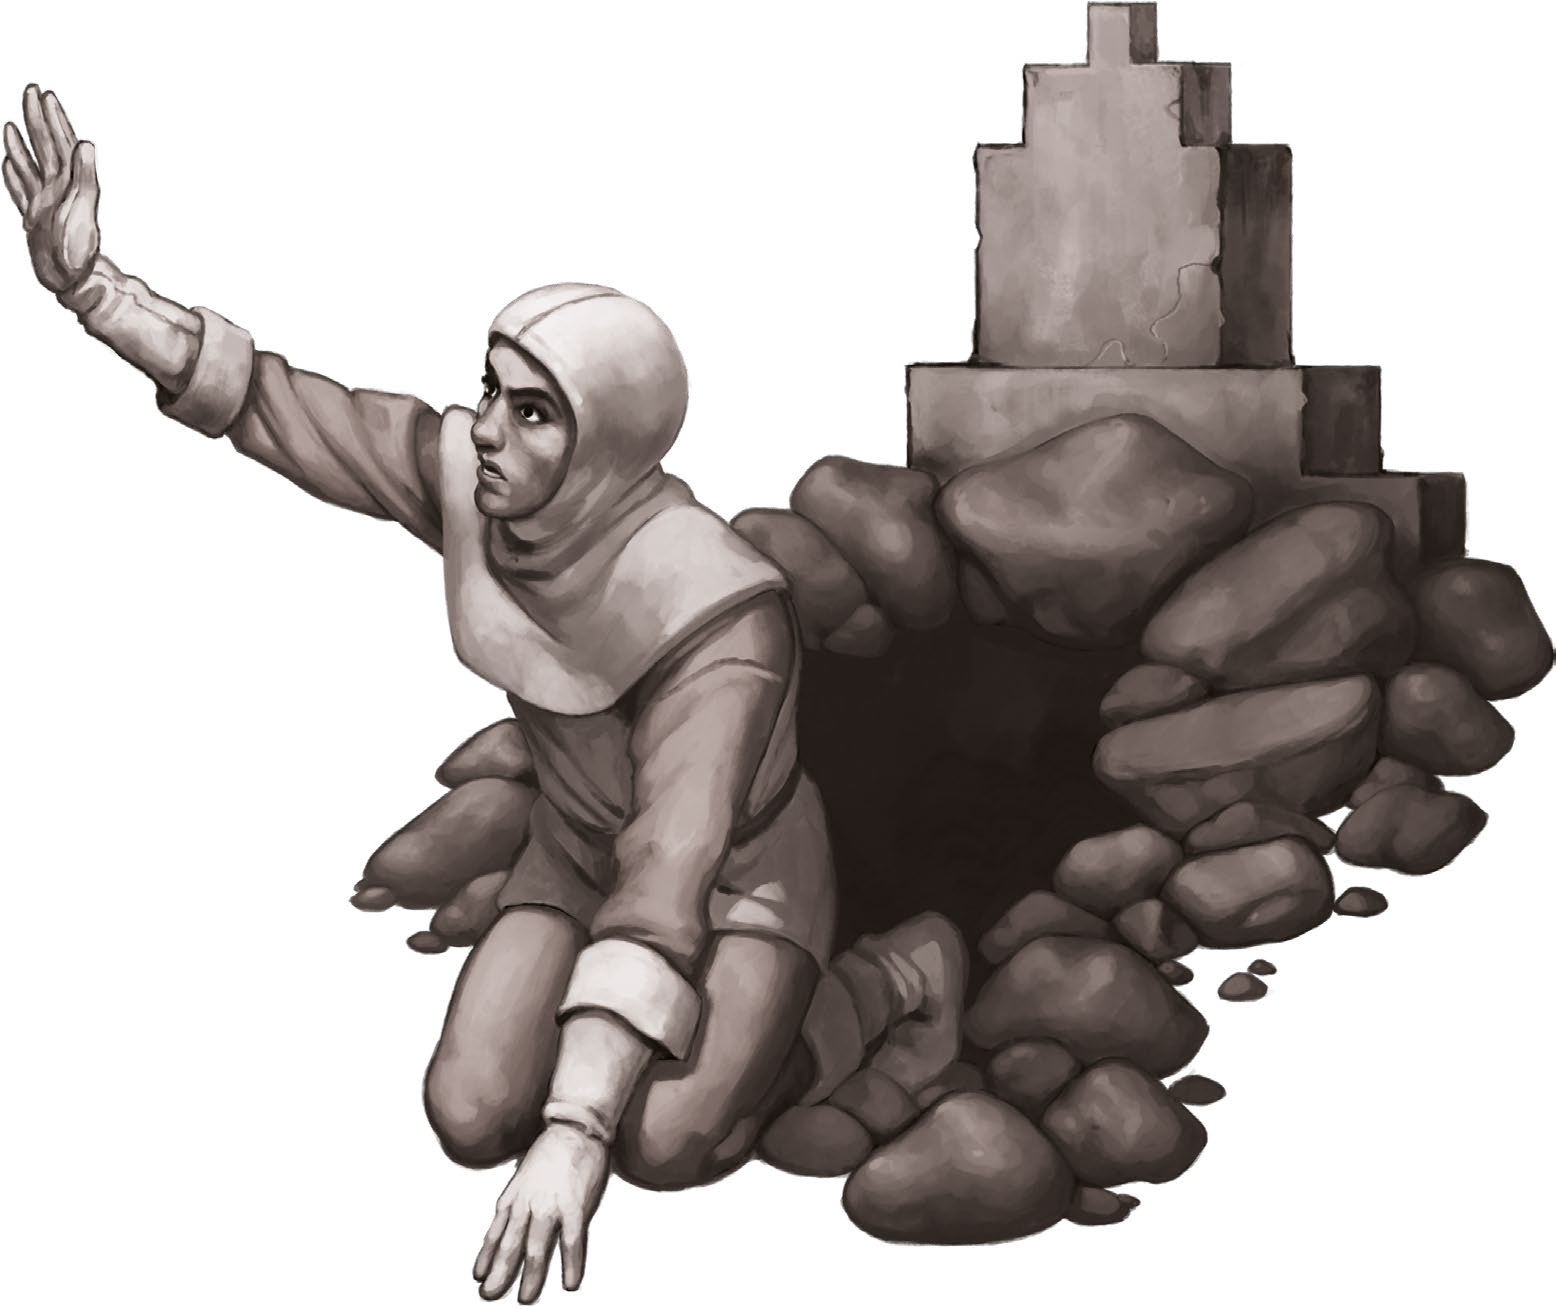
\includegraphics[width=0.65\linewidth]{\art/resurrection.png}
\end{center}

\end{multicols}

\begin{figure*}[!h]
  \mbox{}
  \hfill
  \begin{minipage}[t]{0.44\textwidth}
    \centering
    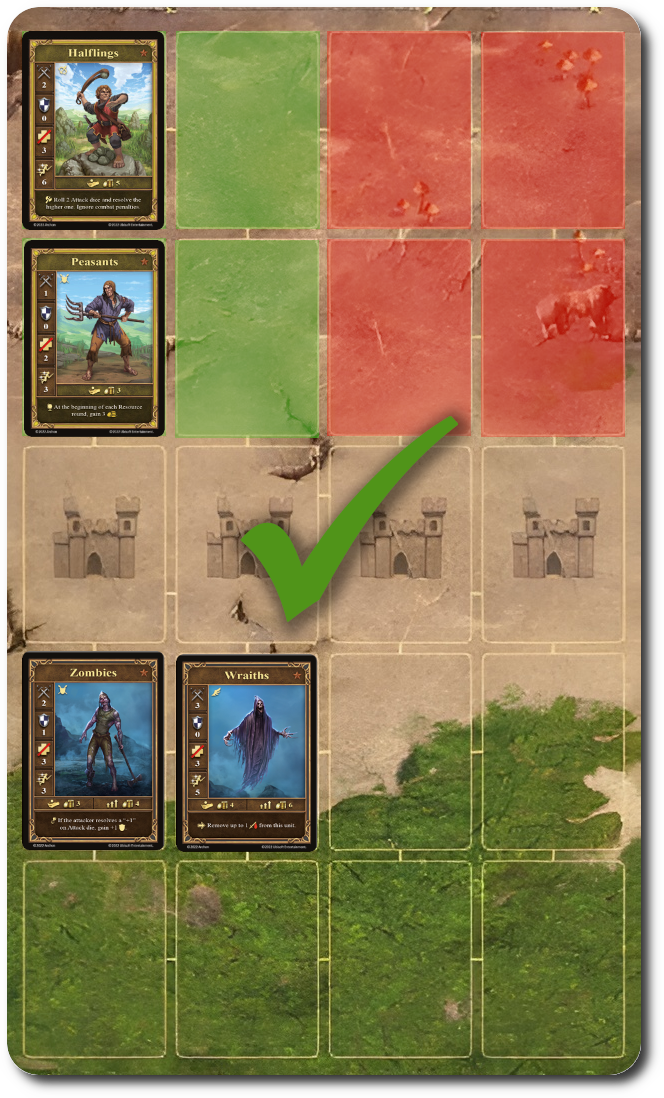
\includegraphics[width=\linewidth]{\examples/battle_good.png}
    \caption[good protected]{\textit{Neutral Units are positioned correctly.}}
  \end{minipage}
  \hfill
  \begin{minipage}[t]{0.44\textwidth}
    \centering
    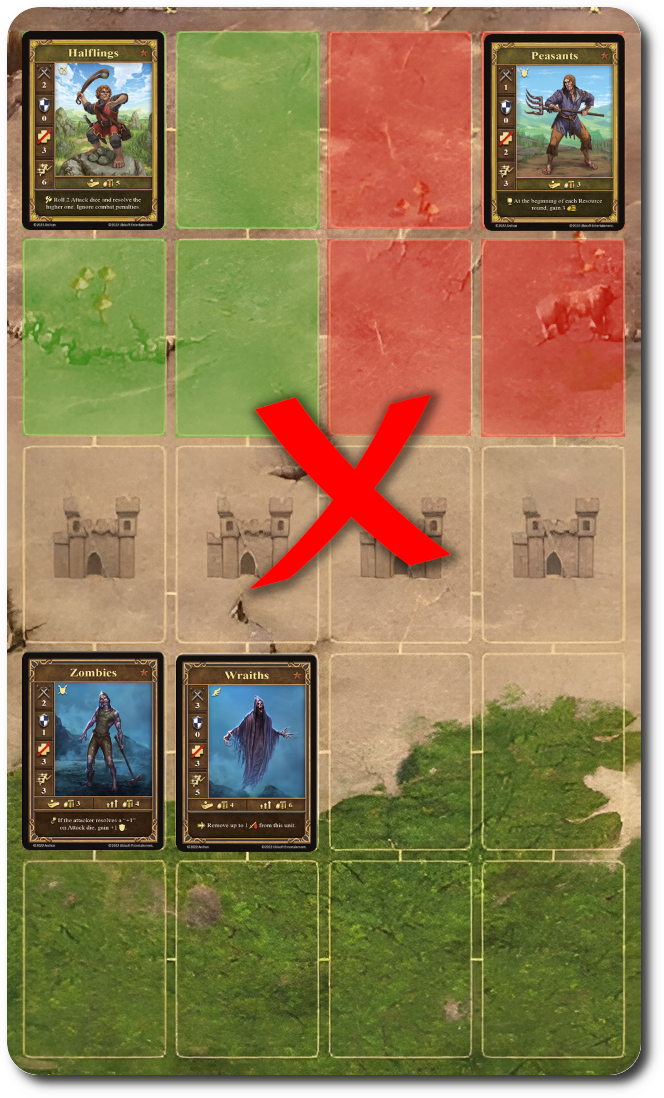
\includegraphics[width=\linewidth]{\examples/battle_bad.png}
    \caption[bad protected]{\textit{This deployment is not allowed because the Necropolis player placed their Units on the left half of the Combat Board.
      The Peasants must also start the Combat on the left side.}}
  \end{minipage}
  \hfill
  \mbox{}
\end{figure*}

\clearpage

\begin{figure*}[!h]
  \mbox{}
  \hfill
  \begin{minipage}[t]{0.44\textwidth}
    \centering
    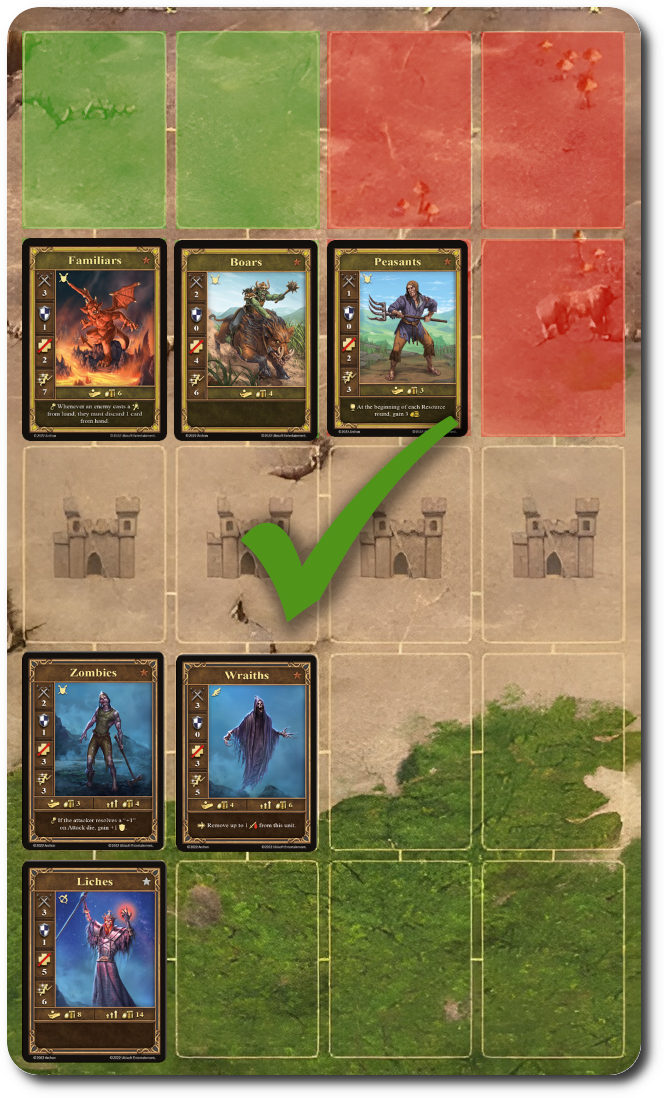
\includegraphics[width=\linewidth]{\examples/battle_exception.png}
    \caption[exception protected]{\textit{\textbf{Exception:} Three non-\svg{unit_ranged} Units must be positioned on the front line.}}
  \end{minipage}
  \hfill
  \begin{minipage}[t]{0.44\textwidth}
    \centering
    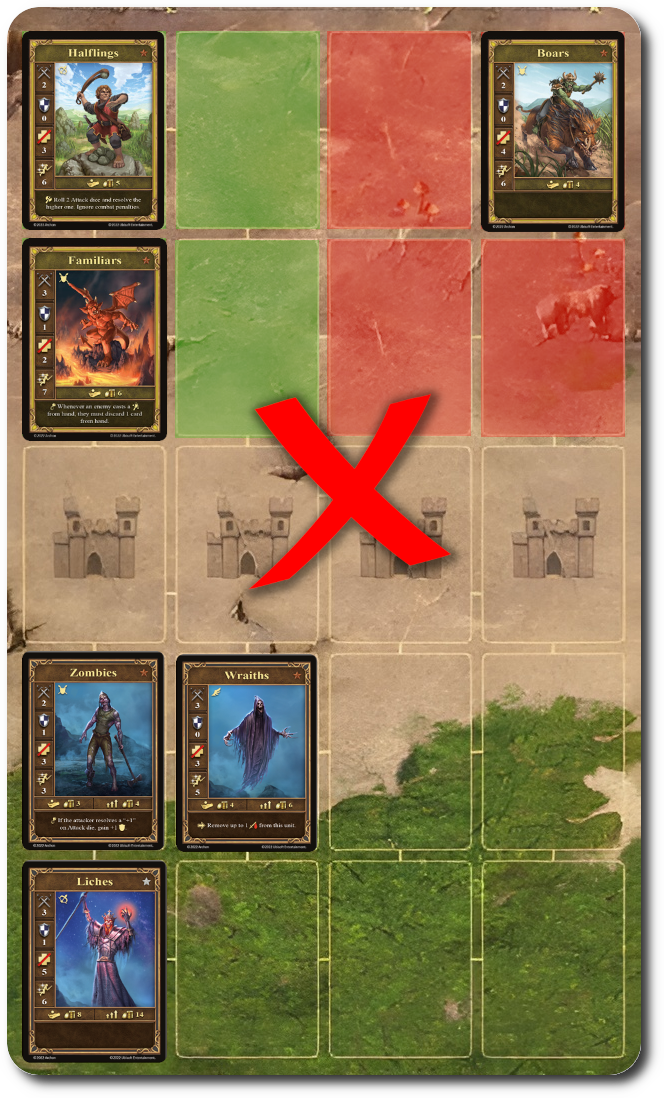
\includegraphics[width=\linewidth]{\examples/battle_ranged_bad.png}
    \caption[ranged protected]{\textit{The Boars must occupy one of the green Fields.}}
  \end{minipage}
  \hfill
  \mbox{}
\end{figure*}

\begin{multicols}{2}

\subsection*{General Recommendations}

The following are not custom rules, but rather recommendations to help you get the most out of your game:

\begin{itemize}
  \item When deciding which building to construct in your Town, especially in the early game, it is \textit{usually} best to prioritize Units over the City Hall, Citadel, Mage Guild, or other Faction-specific buildings.
  \item If you're unsure which Spell, Artifact, or Ability to choose, prioritize those that help you cycle through your Deck.
    This includes any cards that allow you to draw cards or retrieve cards from your Discard Pile.
  \item Try to avoid using your Main Hero's Movement Points for Actions that your Secondary Hero can handle, such as flipping the Map Tiles, Visiting Water Wheels, and so on.
\end{itemize}

\begin{center}
  
\includegraphics[width=0.7\linewidth]{\art/coin.png}
\end{center}

\end{multicols}


% !TeX spellcheck = en_US

\addsection{Credits}{\images/experience.png}

\iftoggle{printable}{\vspace{-\baselineskip}}{}

\bigbreak

\begin{multicols*}{2}

This project shamelessly borrows best practices from the \href{https://github.com/Heegu-sama/Homm3BG}{\textbf{Rule Book Rewrite Project}}, including \LaTeX{} code, GitHub engineering, and translation framework.
You should check it out if you haven't seen it yet.

\textbf{Scenario templating and \LaTeX{} writing}: Tomáš Zeman, Andrzej Wiącek, Saveliy Ivanov

\phantom{Translators placeholder}

\textbf{Special thanks}: Patrick Kersten for \href{https://zedero.github.io/HoMM3BoardgameScenarioEditor/}{Scenario Map Editor}.
Everyone from Archon Studio, for producing the game and answering our incessant queries about rules and other topics.
Jon Van Caneghem and everyone involved with the development of the original video game.
Everyone who has supported the project with suggestions, corrections, image resources, and words of encouragement either on Discord or BoardGameGeek.

\textbf{Artwork borrowed from the official release was made by}: Tomasz Badalski, Yoann Boissonnet, Shen Fei, Viviane Tybusch Souza, Iana Vengerova, Bartosz Winkler

\columnbreak

\vspace*{\fill}


\includegraphics[width=1.3\linewidth]{\art/genie.png}

\vspace*{\fill}

\end{multicols*}


% % % !TeX spellcheck = en_US
\addsection{Notes}{\images/intelligence.png}

\begin{tikzpicture}[remember picture, overlay, blend mode=multiply]
  \node[inner sep=0, opacity=0.44] at (current page.center)
  {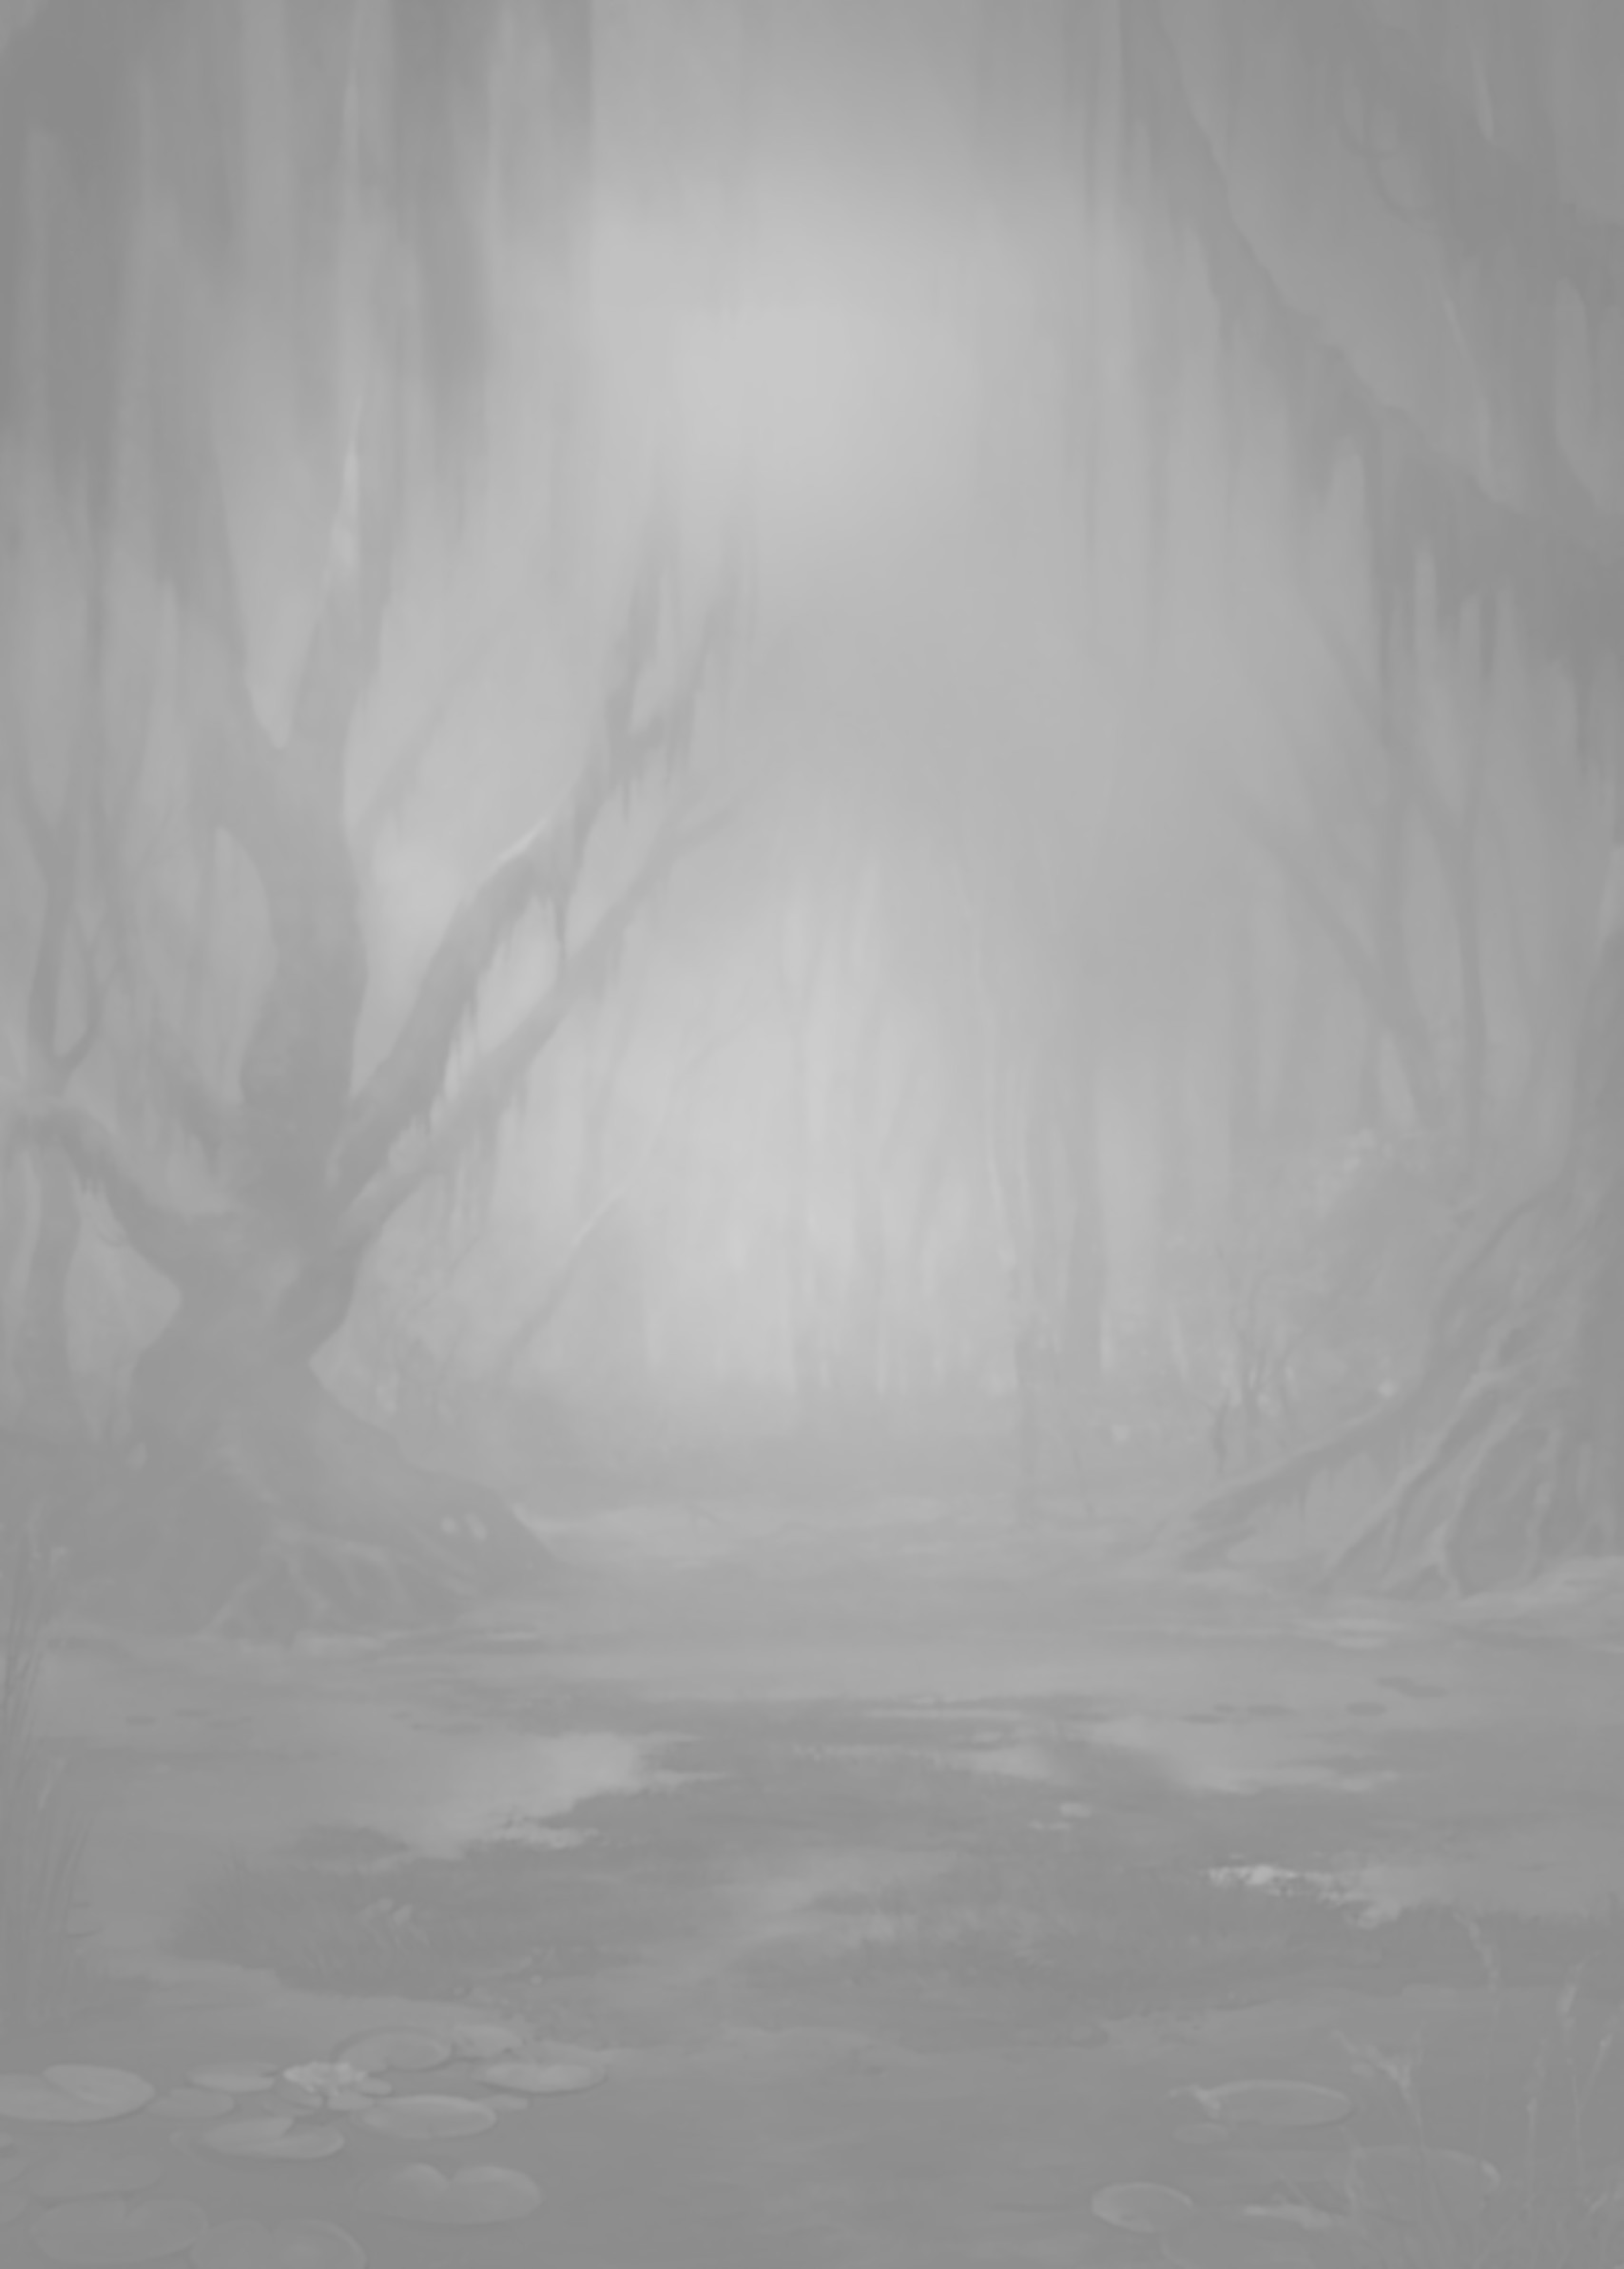
\includegraphics[width=\paperwidth, height=\paperheight]{\layout/citadel_background.jpg}};
\end{tikzpicture}


% !TeX spellcheck = en_US

\restoregeometry

\pagestyle{empty}
\iftoggle{noartbackground}{}{
  \begin{tikzpicture}[remember picture, overlay, inner sep=10pt]
    \node(cover)[anchor=center] at (current page.center) {
      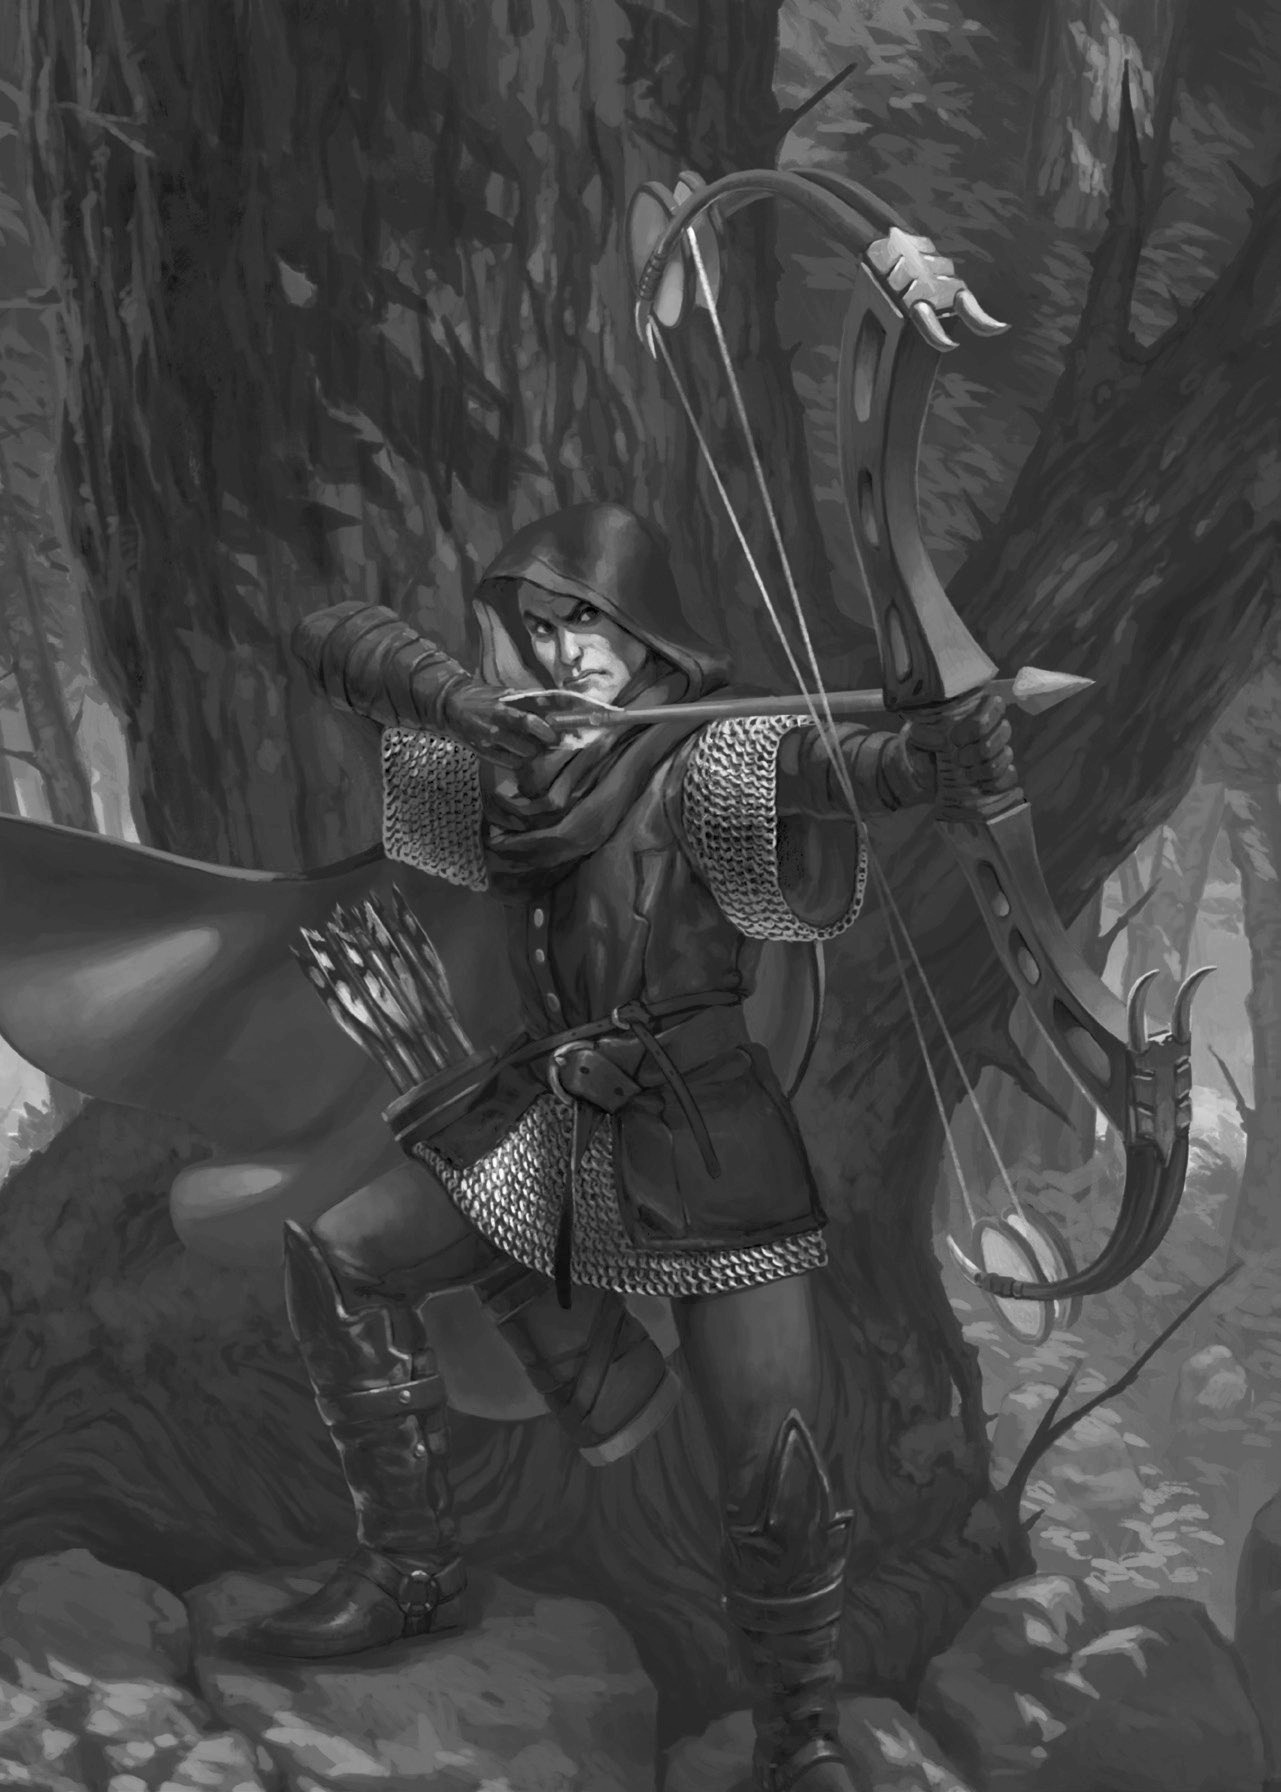
\includegraphics[height=\paperheight, keepaspectratio]{\layout/back.jpg}
    };
  \end{tikzpicture}
}



\iftoggle{individualscenario}{
  % !TeX spellcheck = en_US

\addsection{Got any feedback?}{\images/orb_of_the_firmament.png}

\vspace{\baselineskip}
We hope you enjoyed this scenario.  % no-check-caps
It was created by hobbyists in their free time, for hobbyists just like yourself.
Did you enjoy playing it?
Was there anything that could be improved?
The authors would really appreciate your feedback.
Please reach out using one of the channels below.
Cheers!

\begin{multicols}{2}
  \bigbreak
  \centering
  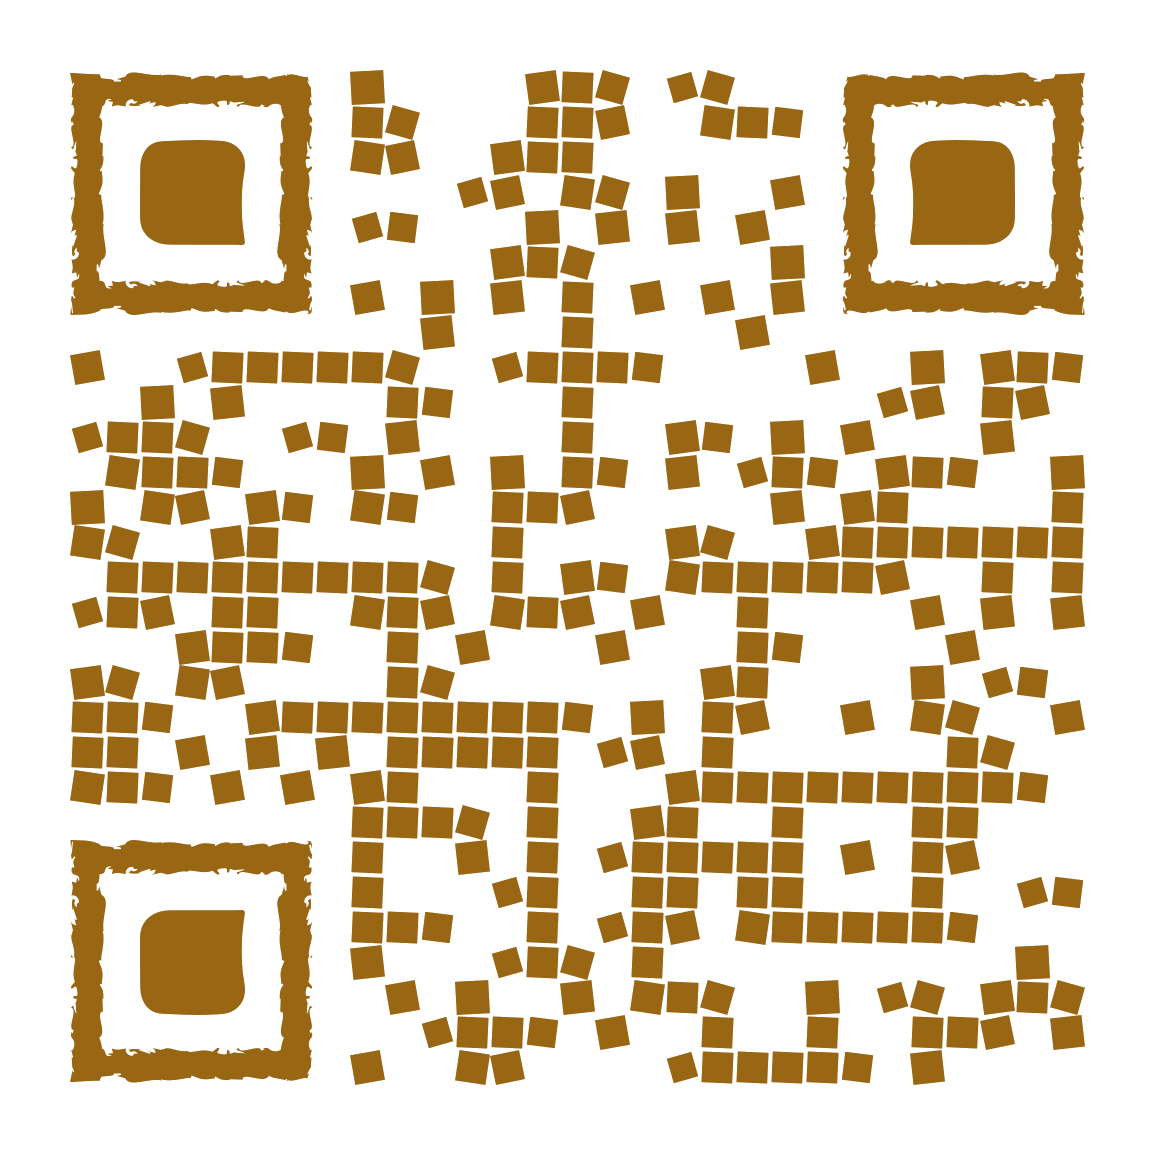
\includegraphics[width=0.8\linewidth]{\qr/discord.png}\\
  Scan to join the Heroes III Board Game community \textbf{Discord} server.\\
  \href{\discordurl}{\discordurl}

  \columnbreak
  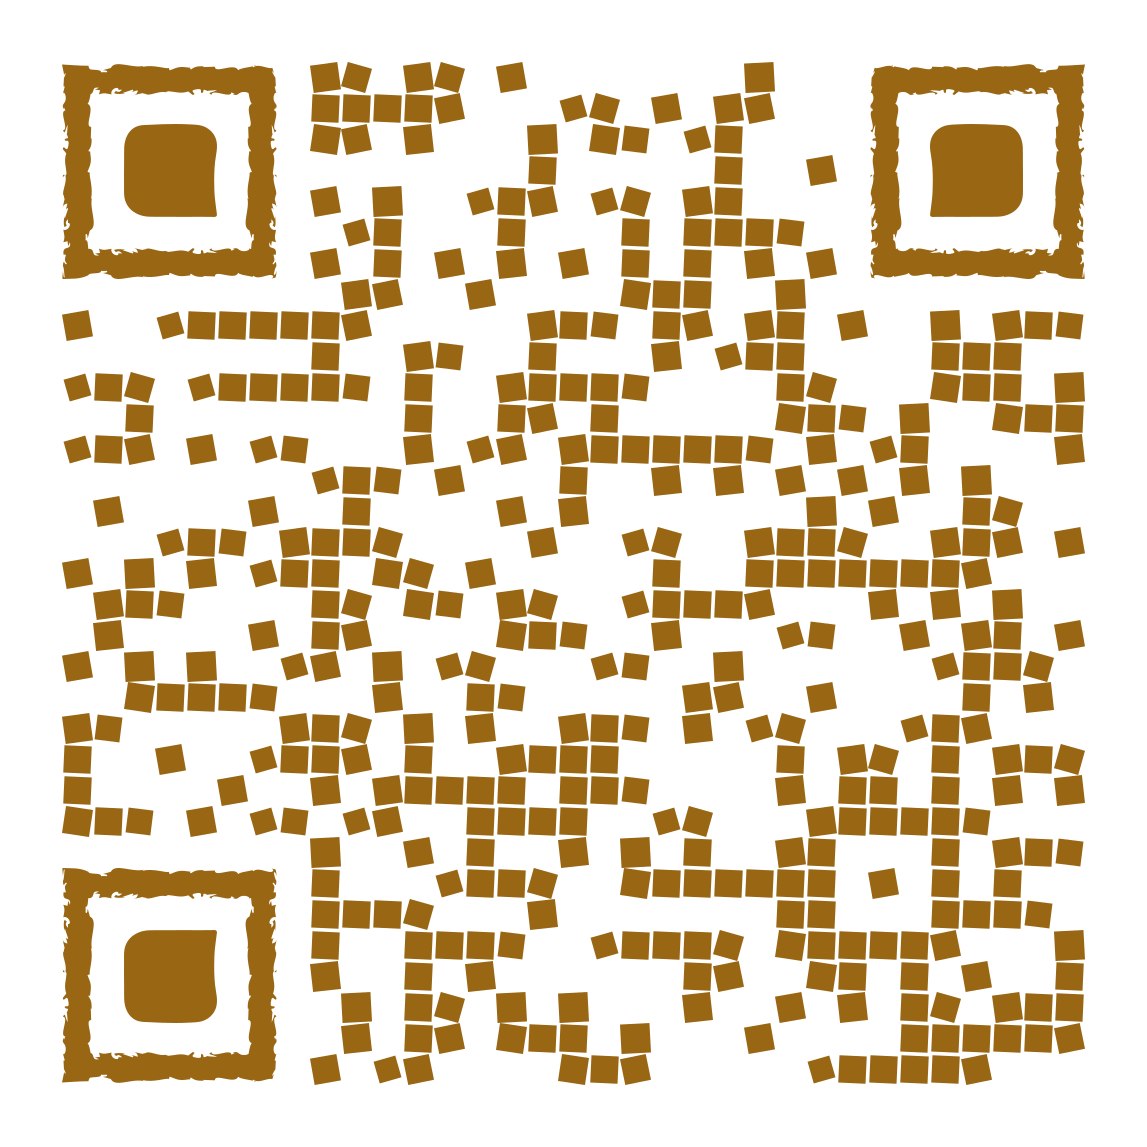
\includegraphics[width=0.8\linewidth]{\qr/github.png} \\
  Scan to open \textbf{GitHub} repository. \\
  \href{\repourl}{\repourl}
\end{multicols}

\vfill
\begin{center}
  \transparent{0.2}{
\includegraphics[width=0.3\linewidth, keepaspectratio]{\art/mirth.png}}
\end{center}

}

\end{document}

